% Options for packages loaded elsewhere
\PassOptionsToPackage{unicode}{hyperref}
\PassOptionsToPackage{hyphens}{url}
%
\documentclass[
  10pt,
]{article}
\usepackage{lmodern}
\usepackage{amssymb,amsmath}
\usepackage{ifxetex,ifluatex}
\ifnum 0\ifxetex 1\fi\ifluatex 1\fi=0 % if pdftex
  \usepackage[T1]{fontenc}
  \usepackage[utf8]{inputenc}
  \usepackage{textcomp} % provide euro and other symbols
\else % if luatex or xetex
  \usepackage{unicode-math}
  \defaultfontfeatures{Scale=MatchLowercase}
  \defaultfontfeatures[\rmfamily]{Ligatures=TeX,Scale=1}
\fi
% Use upquote if available, for straight quotes in verbatim environments
\IfFileExists{upquote.sty}{\usepackage{upquote}}{}
\IfFileExists{microtype.sty}{% use microtype if available
  \usepackage[]{microtype}
  \UseMicrotypeSet[protrusion]{basicmath} % disable protrusion for tt fonts
}{}
\makeatletter
\@ifundefined{KOMAClassName}{% if non-KOMA class
  \IfFileExists{parskip.sty}{%
    \usepackage{parskip}
  }{% else
    \setlength{\parindent}{0pt}
    \setlength{\parskip}{6pt plus 2pt minus 1pt}}
}{% if KOMA class
  \KOMAoptions{parskip=half}}
\makeatother
\usepackage{xcolor}
\IfFileExists{xurl.sty}{\usepackage{xurl}}{} % add URL line breaks if available
\IfFileExists{bookmark.sty}{\usepackage{bookmark}}{\usepackage{hyperref}}
\hypersetup{
  hidelinks,
  pdfcreator={LaTeX via pandoc}}
\urlstyle{same} % disable monospaced font for URLs
\usepackage[left=2cm, right=2cm, top=2cm, bottom=3cm, footskip = .5cm]{geometry}
\usepackage{graphicx,grffile}
\makeatletter
\def\maxwidth{\ifdim\Gin@nat@width>\linewidth\linewidth\else\Gin@nat@width\fi}
\def\maxheight{\ifdim\Gin@nat@height>\textheight\textheight\else\Gin@nat@height\fi}
\makeatother
% Scale images if necessary, so that they will not overflow the page
% margins by default, and it is still possible to overwrite the defaults
% using explicit options in \includegraphics[width, height, ...]{}
\setkeys{Gin}{width=\maxwidth,height=\maxheight,keepaspectratio}
% Set default figure placement to htbp
\makeatletter
\def\fps@figure{htbp}
\makeatother
\setlength{\emergencystretch}{3em} % prevent overfull lines
\providecommand{\tightlist}{%
  \setlength{\itemsep}{0pt}\setlength{\parskip}{0pt}}
\setcounter{secnumdepth}{-\maxdimen} % remove section numbering
% Set up the fonts
\usepackage[urw-palatino]{mathdesign}
\usepackage[T1]{fontenc}


% Set the language for 508
\hypersetup{
  pdftitle = {title},
  pdflang = en-US}

% Add accessibility support from http://www.richschwinn.com/accessibility
\RequirePackage{accsupp}
\RequirePackage{pdfcomment}
\newcommand{\AccTool}[2]{\BeginAccSupp{method=pdfstringdef,unicode,Alt={{#1}}}\pdftooltip{{#2}}{{#1}}\EndAccSupp{}}


% Set up the headers and footers
\usepackage{graphicx}
\usepackage{fancyhdr}
\usepackage{ifthen}
\usepackage{everypage}
\usepackage{float}
\usepackage{subfig}
\usepackage{wrapfig}

% Avoid struggling over figure and table float in Rmarkdown
\let\origfigure\figure
\let\endorigfigure\endfigure
\renewenvironment{figure}[1][2] {
    \expandafter\origfigure\expandafter[H]
} {
    \endorigfigure
}

\let\origtable\table
\let\endorigtable\endtable
\renewenvironment{table}[1][2] {
    \expandafter\origtable\expandafter[H]
} {
    \endorigtable
}

% First page has the large title and NOAA logo
\pagestyle{fancy}
\fancyhf{}
\setlength\headheight{40pt}
\cfoot{\thepage}

\AddEverypageHook{%
   \ifthenelse{\value{page}=1}%
     {\rhead{
\includegraphics[width=40pt]{images/NOAA_logo.png} \\ \textsf{\emph{DRAFT}}}
      \lhead{\textsf{\LARGE State of the Ecosystem 2020: Response Memo}}
      }%
     {\rhead{}
      \lhead{\textsf{\emph{State of the Ecosystem 2020: Response Memo}}}
     }
}

\renewcommand{\headrulewidth}{0.4pt}
\renewcommand{\footrulewidth}{0pt}

% Make caption fonts a bit smaller
\usepackage[font={small}]{caption}


% Change section labels to san serif
\usepackage{sectsty}
\allsectionsfont{\normalfont\sffamily\bfseries}
\usepackage{booktabs}
\usepackage{longtable}
\usepackage{array}
\usepackage{multirow}
\usepackage{wrapfig}
\usepackage{float}
\usepackage{colortbl}
\usepackage{pdflscape}
\usepackage{tabu}
\usepackage{threeparttable}
\usepackage{threeparttablex}
\usepackage[normalem]{ulem}
\usepackage{makecell}
\usepackage{xcolor}

\author{}
\date{\vspace{-2.5em}}

\begin{document}

\hypertarget{introduction}{%
\section{Introduction}\label{introduction}}

In the table below we summarize all comments and requests with sources.
The Progress column briefly summarizes how we responded, with a more
detailed response in the numbered Memo Section. In the Progress column,
``SOE'' indicates a change included in the report(s).

\begingroup\fontsize{9}{11}\selectfont

\begin{longtable}{>{\raggedright\arraybackslash}p{5cm}>{\raggedright\arraybackslash}p{2cm}>{\raggedright\arraybackslash}p{5cm}>{\raggedright\arraybackslash}p{2cm}}
\toprule
\textbf{Request} & \textbf{Source} & \textbf{Progress} & \textbf{Memo Section}\\
\midrule
\endfirsthead
\multicolumn{4}{@{}l}{\textit{(continued)}}\\
\toprule
\textbf{Request} & \textbf{Source} & \textbf{Progress} & \textbf{Memo Section}\\
\midrule
\endhead
\
\endfoot
\bottomrule
\endlastfoot
\rowcolor{gray!6}  Formal response to requests & Both Councils & this response memo & Introduction\\
Consider report card like Alaska's & Both Councils & SOE summary bullets (page 1) & 1\\
\rowcolor{gray!6}  Include summary visualization & Both Councils & SOE infographics (page 2) & 2\\
Include uncertainty estimates for all indicators & Both Councils & SOE survey biomass uncertainty included; feedback requested for other indicators & 3\\
\rowcolor{gray!6}  Include Downeast ME (Scotian Shelf EPU) & NEFMC & SOE survey biomass now includes most of downeast ME; human dimensions include downeast ME & 4\\
Link zooplankton abundance and or community composition to fish condition & NEFMC & SOE page 2 research spotlight & 5\\
\rowcolor{gray!6}  Ocean acidification information & Both Councils & work in progress to develop baseline and monitoring & 6\\
Gulf Stream Index/Labrador current interaction & Both Councils & SOE Labrador current and Gulf Stream indices now included in both reports & 7\\
\rowcolor{gray!6}  Include source for PP estimates (satellite vs in situ) & NEFMC & SOE clarified that all PP estimates are from satellite & 8\\
Shellfish growth/distribution linked to climate (system productivity) & MAFMC & project with R. Mann student to start late 2020 & 9\\
\rowcolor{gray!6}  Estuarine condition relative to power plants and temp & MAFMC & inadequate resourses to address this year & 10\\
Frequency and occurrence of warm core rings & MAFMC & SOE added indicator & 11\\
\rowcolor{gray!6}  Cold pool index & MAFMC & SOE added indicator & 12\\
Nutrient inputs and water quality near shore & MAFMC & SOE Chesapeake update; summary of data from National Estuarine Research Reserve network started, example info included here & 13\\
\rowcolor{gray!6}  Link environmental and social, economic indicators & NEFMC & SOE PP required, habitat and wind overlap, page 2 conceptual model & 14\\
Quantitative overlap of wind area and habitat and fishing areas & MAFMC & SOE habitat wind overlap, wind overlap with fisheries for next round & 15\\
\rowcolor{gray!6}  Include links to Social Science websites & NEFMC & SOE link included in both reports & 16\\
Management complexity & MAFMC & project started by summer student in 2018, needs further analysis & 17\\
\rowcolor{gray!6}  South Atlantic Council managed species represented in recreational indices & MAFMC & SOE revised indicator and noted change in report & 18\\
Add social elements from overview conceptual model to NE conceptual model & NEFMC & older general conceptual model replaced by specific links between indicators in report & 19\\
\rowcolor{gray!6}  Avg. weight of diet components by feeding group, mean stomach weight across feeding guilds & Both Councils & stomach fullness analysis started--species level; feedback requested & 20\\
North Atlantic Right Whale calf production indicator & NEFMC & SOE added indicator & 21\\
\rowcolor{gray!6}  Distinguish managed species in report & NEFMC & SOE Council managed species separated in landings figures & 22\\
Marine Mammal consumption & MAFMC & SOE added discussion of seal diets & 23\\
\rowcolor{gray!6}  Small pelagic abundance & MAFMC & SOE have survey planktivore time series but would like to improve; see also SOE forage energy density & 24\\
Young of Year index from multiple surveys & MAFMC & SOE fish production from NEFSC trawl; feedback reqested on how to expand & 25\\
\rowcolor{gray!6}  Biomass of sharks & MAFMC & HMS provided landings for 3 years and working on full time series, still looking for source of biomass data & 26\\
Diversity metric for NEFSC trawl survey & NEFMC & need to reconcile different survey vessel catchabilites or split by vessel & 27\\
\rowcolor{gray!6}  Ecosystem risk score & MAFMC & SOE PP required, marine heat waves are steps towards this; feedback requested for other desired analyses & 28\\
Inflection points for indicators & Both Councils & inadequate resources to do inflection point and threshold analysis this year & 29\\*
\end{longtable}
\endgroup{}

\hypertarget{responses-to-comments}{%
\section{Responses to comments}\label{responses-to-comments}}

\hypertarget{section}{%
\subsection{1}\label{section}}

Both Councils asked for a summary ``report card'' similar to that used
in Alaska {[}\protect\hyperlink{ref-zador_ecosystem_2016}{1}{]}. The
first page of this year's SOE reports summarizes the key messages with
icons showing the message theme (e.g., commercial fisheries, fishing
communities, forage species, system productivity, etc). At present, we
synthesized key findings on both existing and new indicators. We welcome
suggestions for indicators that should always be tracked in this
section, and for further refinements to make this summary more useful.

\hypertarget{section-1}{%
\subsection{2}\label{section-1}}

Both Councils asked for a summary visualization. The first page of the
SOE report uses icons developed to help visualize different report
components. The second page of this year's SOE report has both a map
visualizing the key oceanographic features mentioned in the report along
with fishing communities, and a conceptual model visualizing potential
linkages between report indicators. The conceptual model is discussed
further under point 5 below.

\hypertarget{section-2}{%
\subsection{3}\label{section-2}}

Both Councils asked for uncertainty estimates to be included with
indicators. As a first step, we included survey design-based uncertainty
estimates\footnote{\url{https://noaa-edab.github.io/tech-doc/survdat.html}}
for all surveys where we had haul specific information (all but the
inshore ME-NH survey). Including this uncertainty led to a different
approach to the data, looking for true departures from expected stable
dynamics at the functional group level, and provided insight into which
trends were potentially noteworthy. Survey biomass uncertainty is
included in each SOE (p.~MAFMC and p.~NEFMC).

We experimented with a model-based estimate of uncertainty for survey
biomass which accounts for both spatial and temporal sources (VAST;
{[}\protect\hyperlink{ref-thorson_guidance_2019}{2}{]}). The results are
promising (Fig. \ref{fig:VASTtest}), and may serve not just as a biomass
indicator but also an indicator of distribution shifts for species and
functional groups. This method can also potentailly combine the inshore
and offshore surveys into a single analysis. If the SSCs and Councils
consider this approach promising, we will persue it further for next
year.

\begin{figure}

{\centering 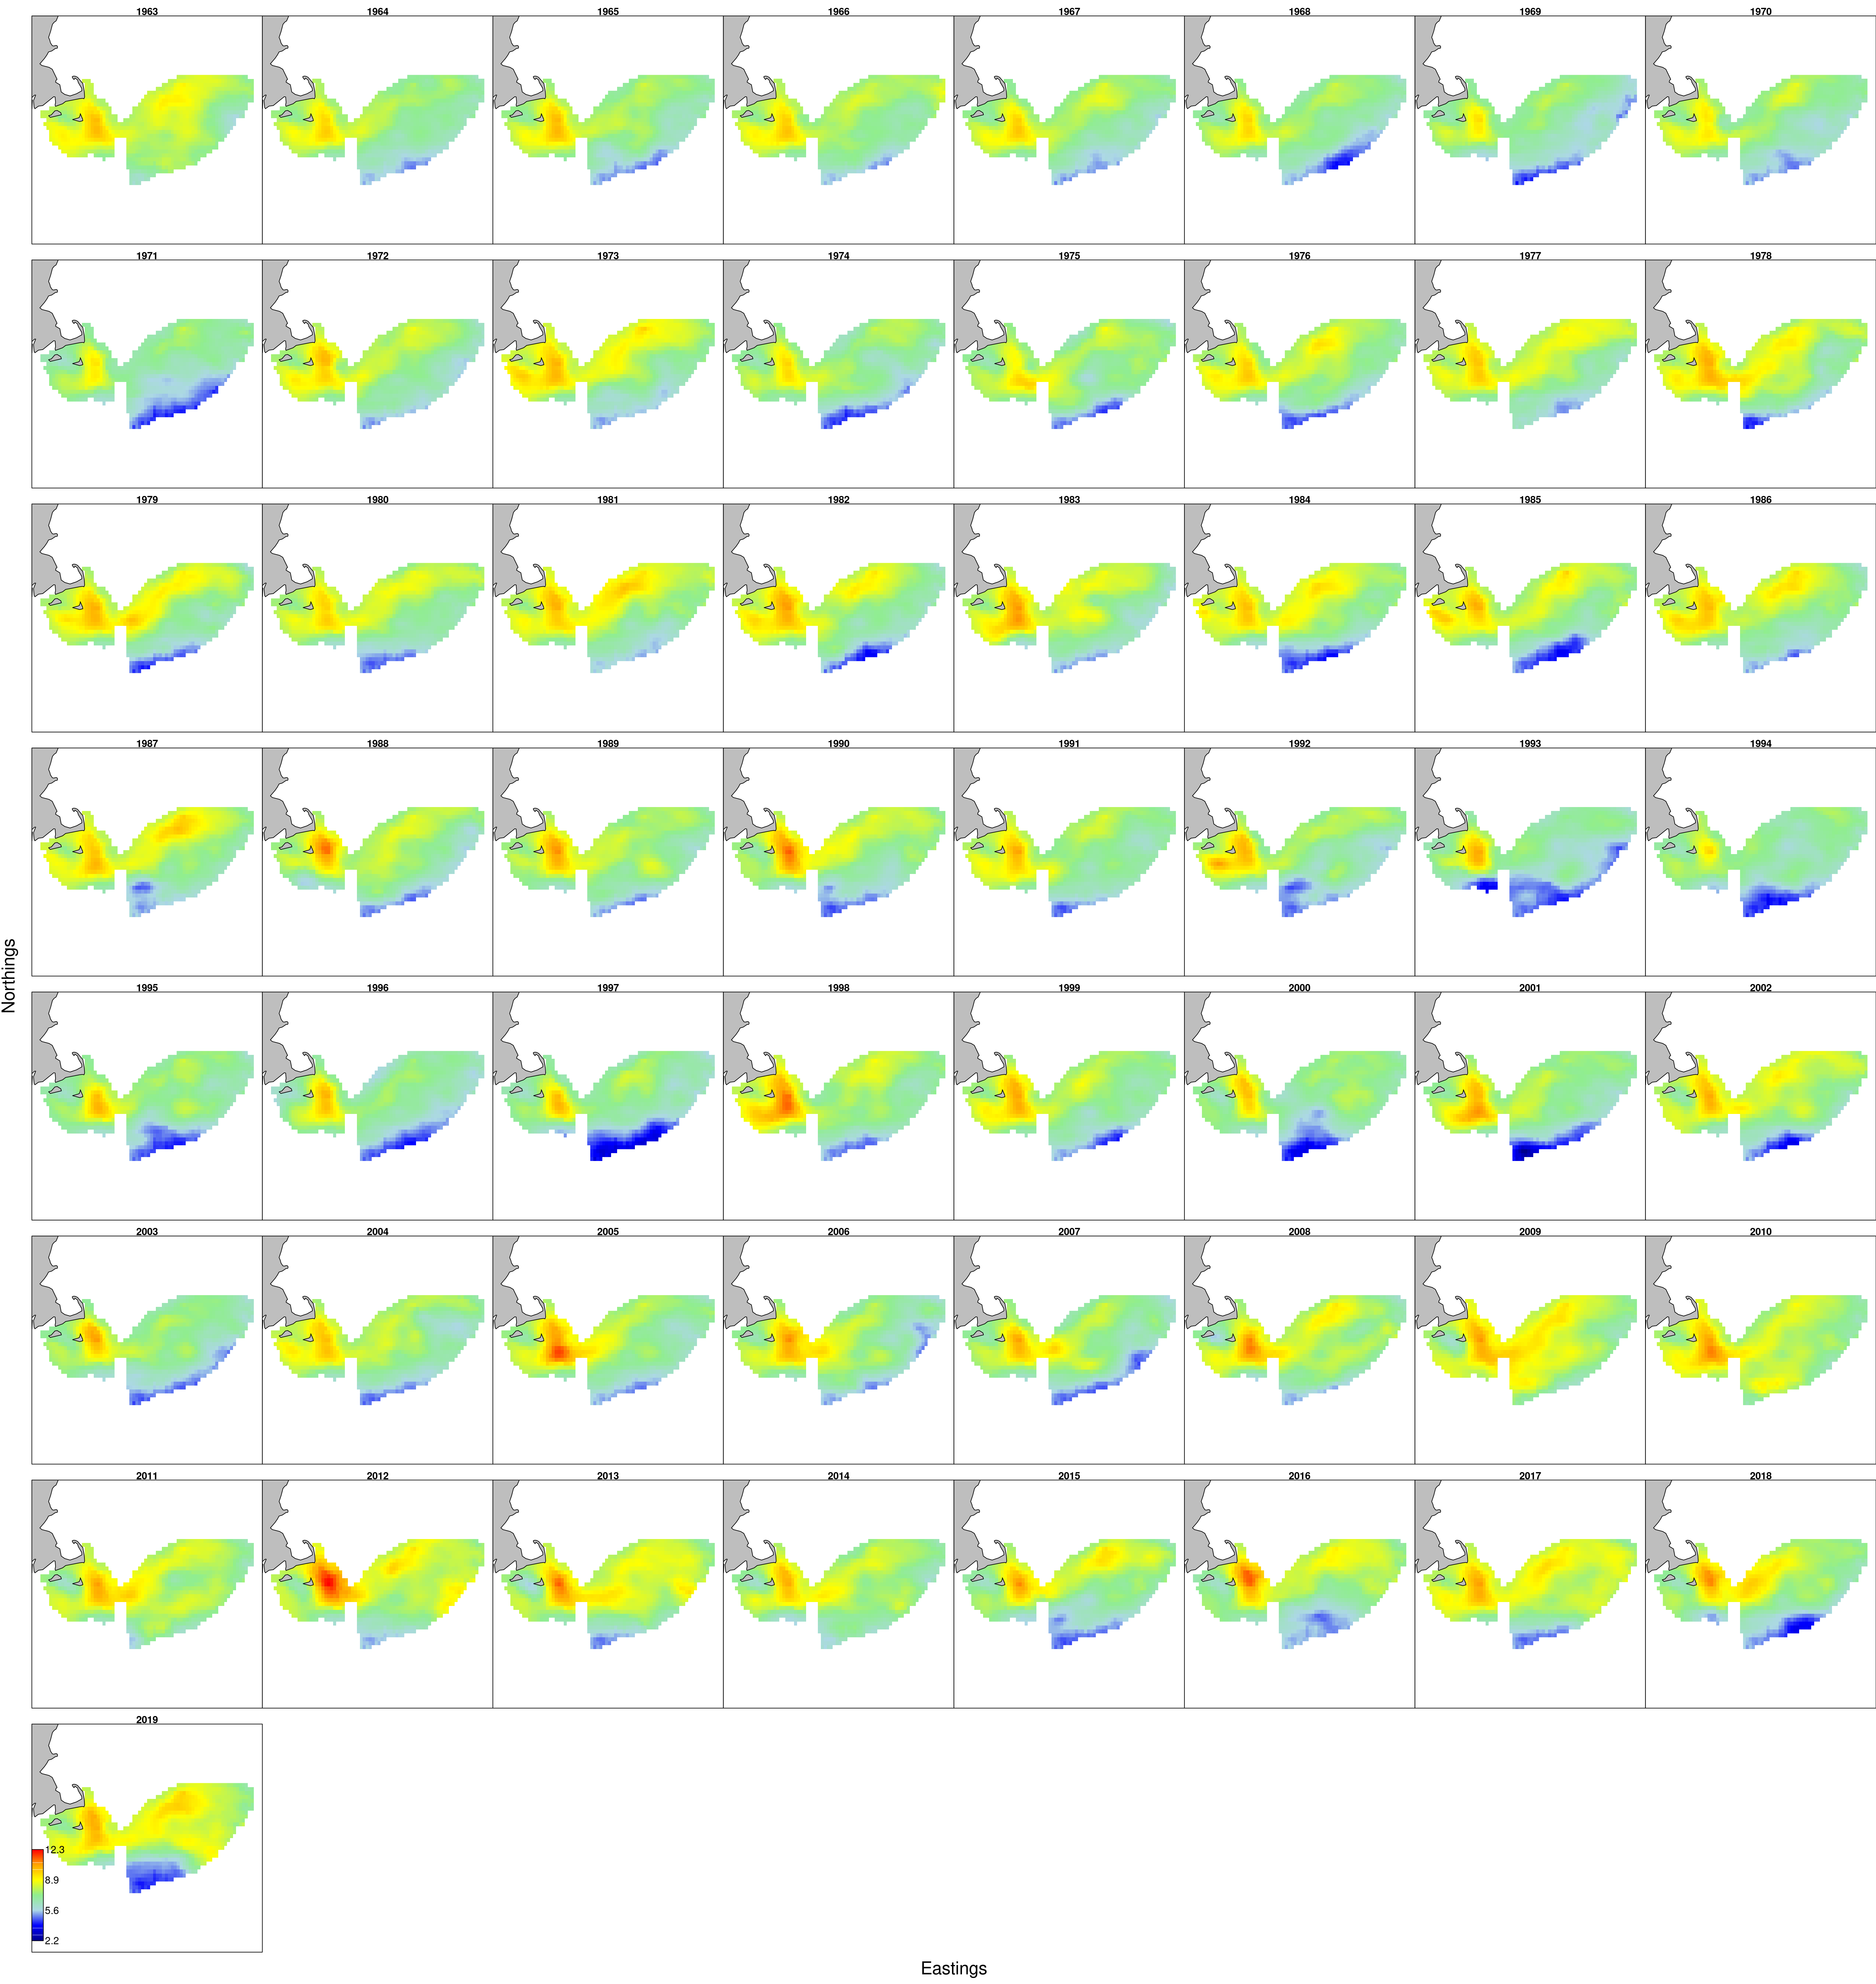
\includegraphics[width=0.49\linewidth]{images/ln_density} 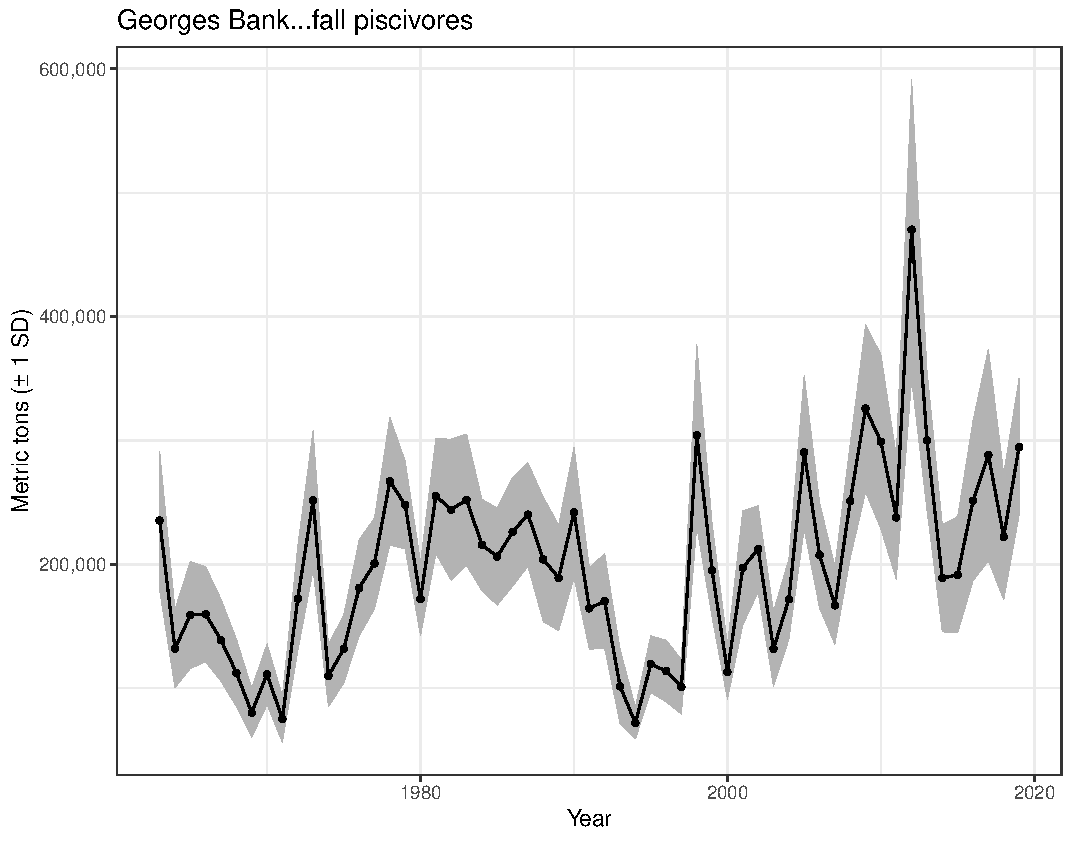
\includegraphics[width=0.49\linewidth]{images/biomass_plot} 

}

\caption{Georges Bank piscivoves biomass and uncertainty as estimated by the VAST model.}\label{fig:VASTtest}
\end{figure}

Some indicators (e.g.~total landings) may have uncertainty which is
difficult to calculate (e.g.~based on unknown reporting errors). Many
other current indicators do not have straightforward uncertainty
calculaltions (e.g.~diversity indices, anomalies) so we welcome
suggestions from the SSC and Council to guide estimation for future
reports.

\hypertarget{section-3}{%
\subsection{4}\label{section-3}}

The NE SSC asked to include downeast ME in future reports, because the
Scotian Shelf EPU which includes downeast ME has not been included in
previous reports. We felt it was inappropriate to report on the Scotian
Shelf EPU, which includes Canadian waters and is an incomplete portion
of the full Soctian Shelf. However, this year we recalculated survey
biomass using an updated strata set that includes much of downeast ME
for the NEFSC (Fig. \ref{fig:survbio-strata}; p.~NEFMC SOE). The inshore
strata not included in the NEFSC trawl survey biomass are represented in
the ME-NH survey (p.~NEFMC SOE) Further, fishery catch and revenue data,
fishing community data, and recreational indicators have always included
downeast ME because both fishing statistical areas and human community
data include all of ME. Therefore, fishery and fish biomass information
reflects much of the area.

\begin{figure}

{\centering 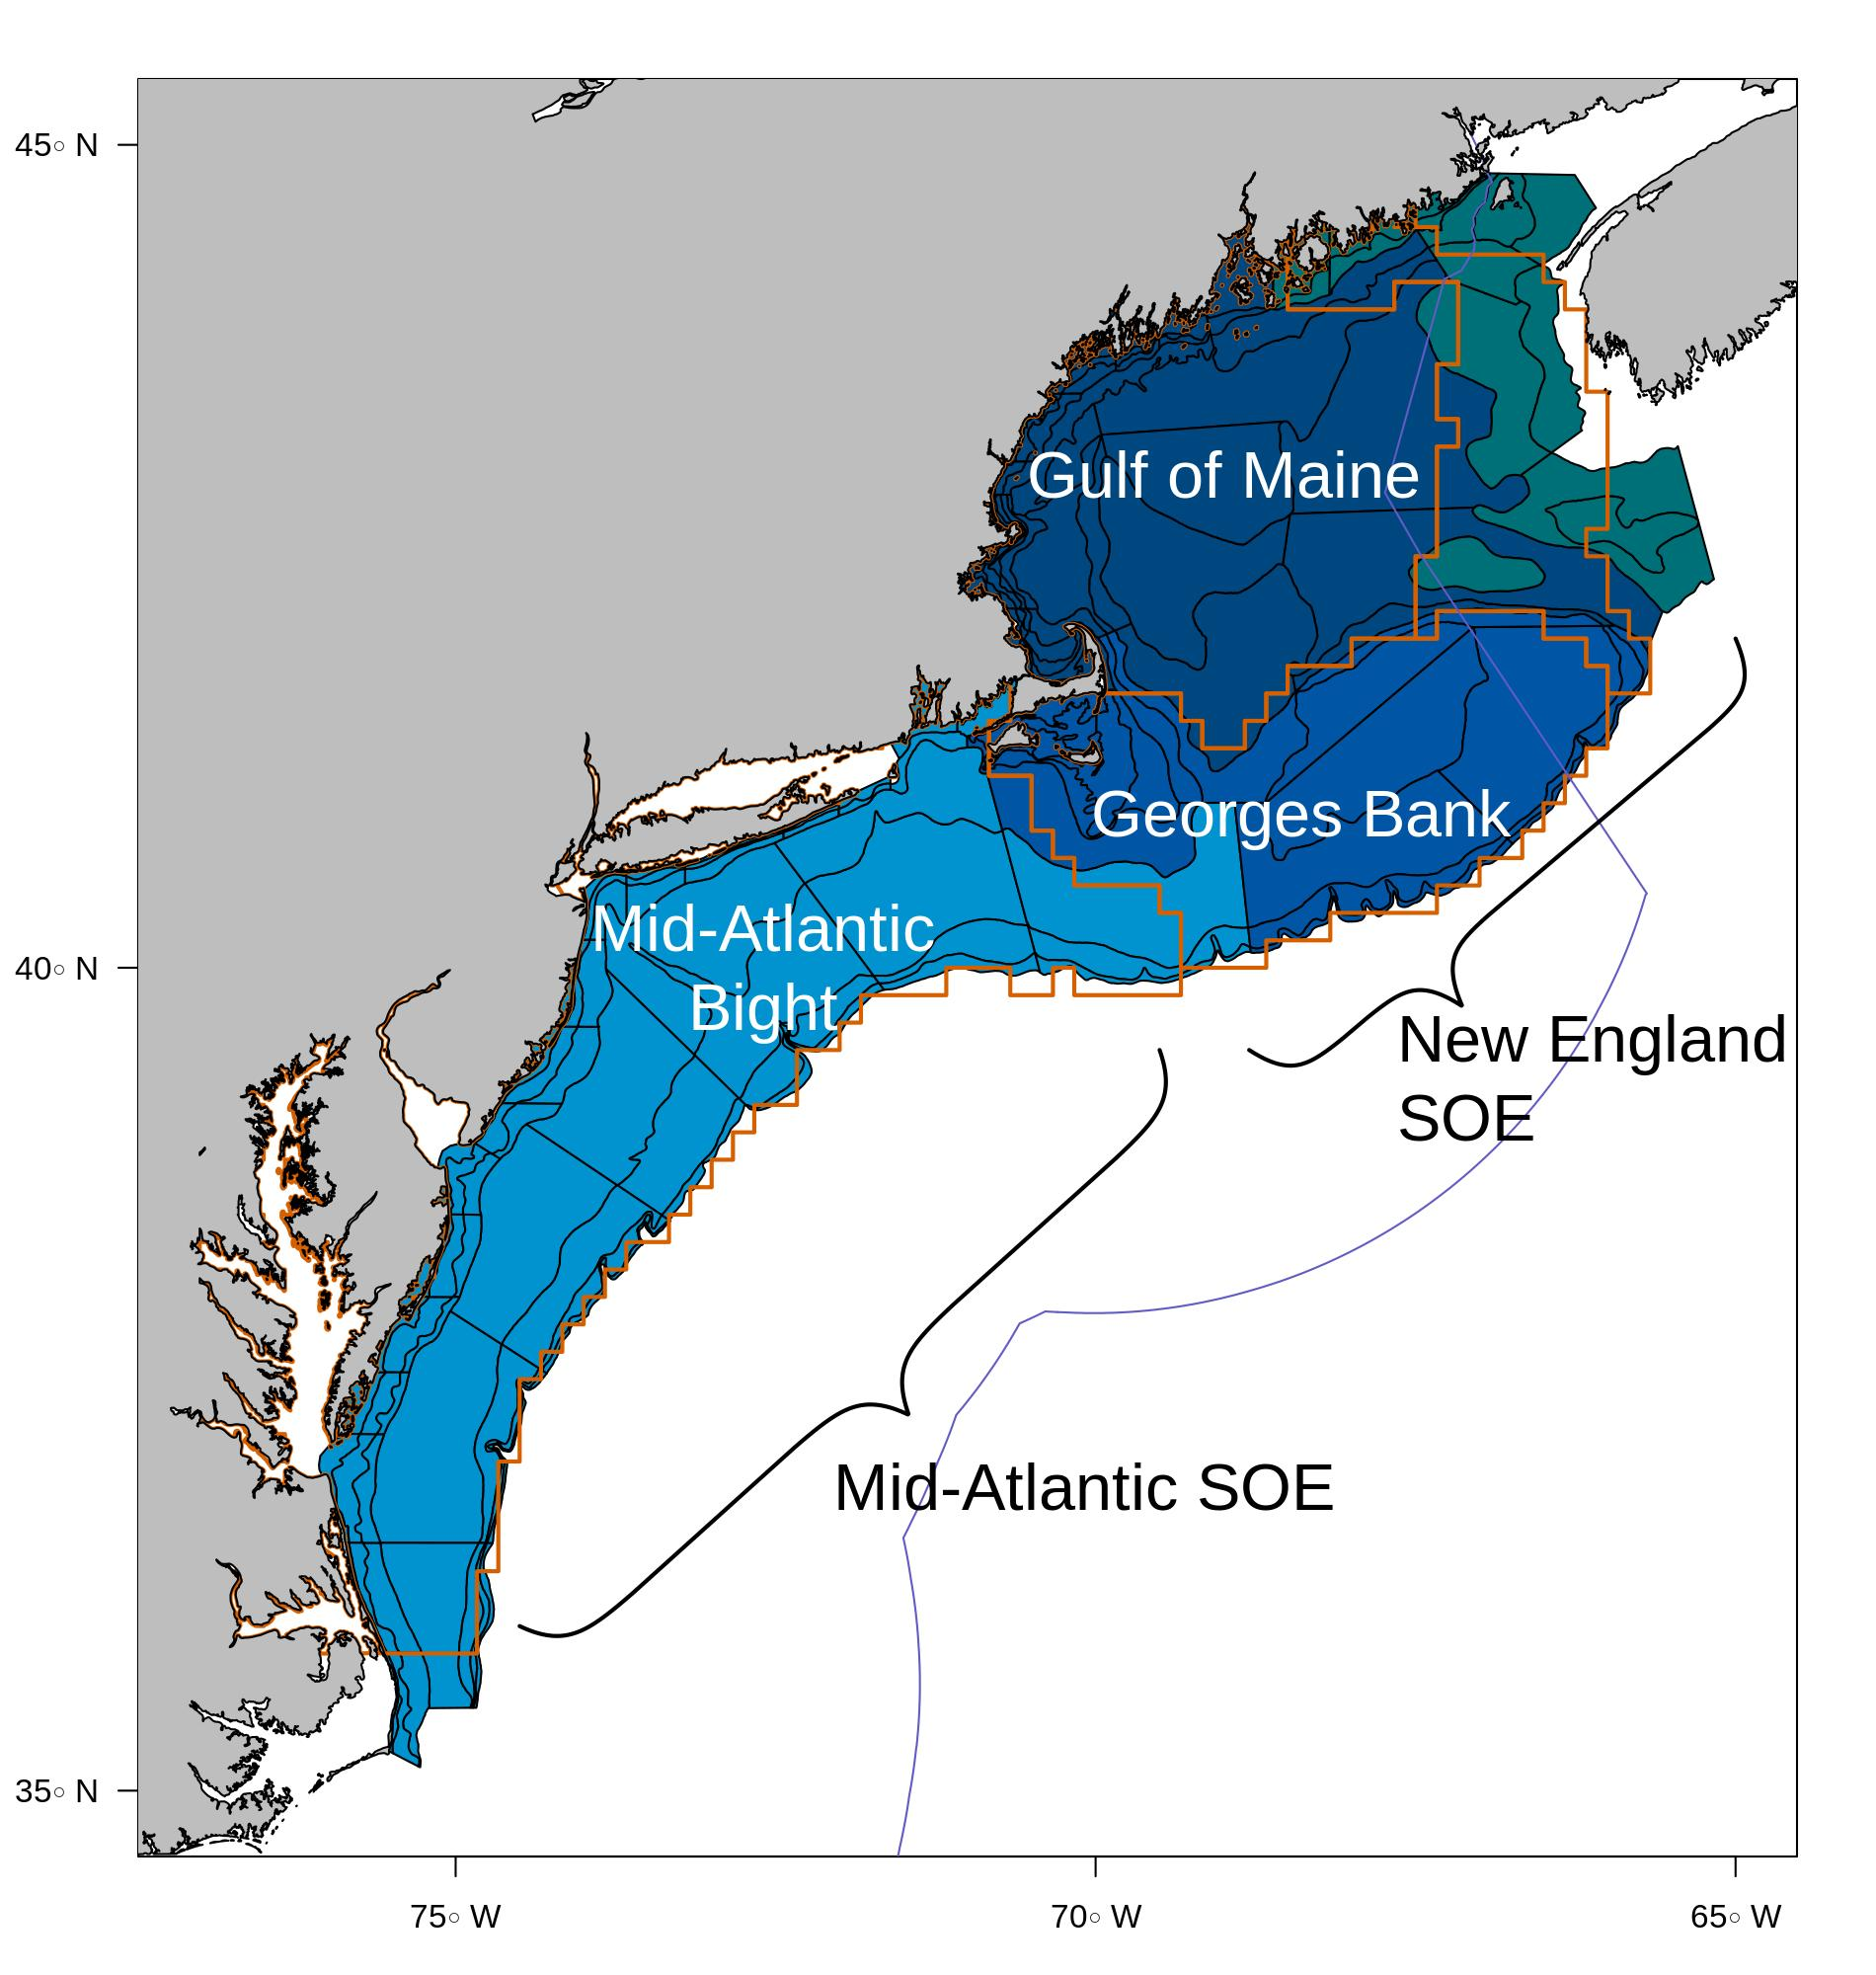
\includegraphics[width=0.8\linewidth]{images/EPU_Designations_Map} 

}

\caption{Survey strata mapping to EPUs for biomass estimates}\label{fig:survbio-strata}
\end{figure}

Oceanographic indicators (surface and bottom temperature, phytoplankton,
zooplankton) remain at the EPU level. The EPUs were defined based on
these characteristics\footnote{\url{https://noaa-edab.github.io/tech-doc/epu.html}}
so we are hesitant to alter them for these indicators without a more
thorough examination of the EPU definitions in general.

\hypertarget{section-4}{%
\subsection{5}\label{section-4}}

Both Councils have been interested in ecosystem energy flow and how
changes in ecosystem productivty link to fishery production. In
particular, the NE SSC asked about further links between zooplankton
abundance and or community composition to fish condition. Research was
initiated during 2019 evaluating statistical relationships between
environmental indicators including temperature, depth, and zooplankton
community composition and fish condition. Initial results are noted in
each SOE (p.~MAFMC and p.~NEFMC). Further work is ongoing to link more
of the indicators in the report using both statistical analysis and
potentially structural equation modeling as noted on p.~2 of each SOE
under ``Research Spotlight.'' This conceptual model shows the full range
of potential linkages, but we plan to start with a subset of linkages
(Fig. \ref{fig:researchlinks}). In particular, potential linkages
between zooplankton and forage fish energy content (p.~MAFMC and
p.~NEFMC) may also be explored in the upcoming years.

\begin{figure}

{\centering 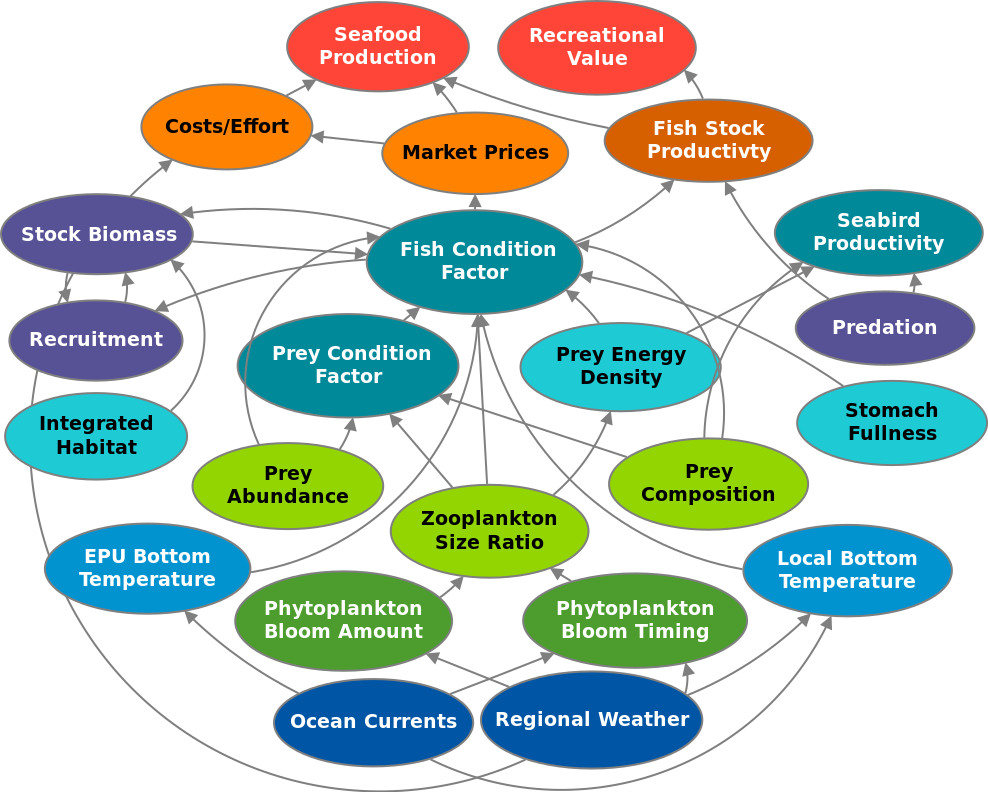
\includegraphics[width=0.49\linewidth]{images/SOEconditionfactorlinks_color} 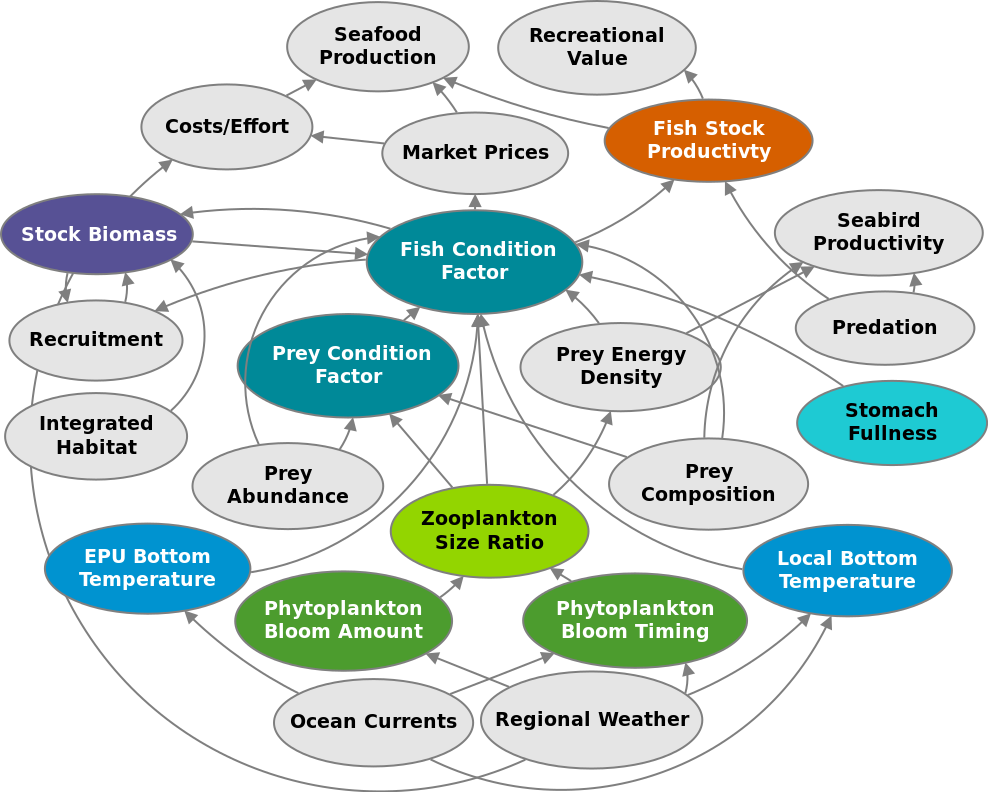
\includegraphics[width=0.49\linewidth]{images/SOEconditionfactorlinks_keycolor} 

}

\caption{Full set of hypothesized relationships between SOE indicators related to fish condition (left) and subset to be investigated first (right).}\label{fig:researchlinks}
\end{figure}

\hypertarget{section-5}{%
\subsection{6}\label{section-5}}

Both Councils asked for information on ocean acidification (OA). In
2019, NOAA reviewed available OA information and is now finalizing a
research plan\footnote{\url{https://sab.noaa.gov/sites/SAB/Meetings/2019_Documents/Dec_Meeting/2020\%20OA\%20Research\%20Plan\%20DRAFT\%20External\%20Review.pdf}}
to address OA comprehensively. Unfortunately, this synthesis was not
available in time to include in the 2020 SOE.

The main message of this forthcoming report is that we don't have much
of a time series of OA monitoring data for our region yet, but we have
been (and will continue) collecting data in the Northeast and that NOAA
sees OA monitoring as a priority. There are three main research
objectives for 2020-2029 outlined in the report:

\begin{enumerate}
\def\labelenumi{\arabic{enumi}.}
\tightlist
\item
  Document and predict change via monitoring, analysis, and modeling.\\
\item
  Characterize and predict biological sensitivity of species and
  ecosystems.\\
\item
  Understand human dimensions and socioeconomic impacts of OA.
\end{enumerate}

Specific work is in progress now and should be available for future SOE
reports, including:

\begin{itemize}
\tightlist
\item
  Aleck Wang (WHOI) and Chris Melrose (NEFSC) are working on climatology
  of spatial and seasonal patterns of carbonate chemistry parameters on
  the Northeast U.S. Continental Shelf, which will form a critical
  baseline for future OA indicators.
\item
  Grace Saba (Rutgers) is the lead PI on a new project which is using
  gliders to characterize OA conditions and to validate/improve OA
  models for the region.
\item
  There is ongoing experimental work being conducted at the NEFSC
  Milford lab that we could include if the information is relevant
\end{itemize}

Until a climatology and time series of OA measurements is available for
comparison, we can include other information on OA in the SOE as it
becomes available. We welcome feedback and suggestions from the SSC and
Council on what information would be most useful.

\hypertarget{section-6}{%
\subsection{7}\label{section-6}}

Both Councils were interested in large scale ocean current interactions
and requested additional information on the Gulf Stream Index and
Labrador current. We have expanded this section and included information
on both Gulf Stream warm core rings (see point 11) and on the decreasing
proportion of Labrador Current water entering the Gulf of Maine in both
SOE reports this year (p.~MAFMC and p.~NEFMC).

\hypertarget{section-7}{%
\subsection{8}\label{section-7}}

The NE SSC asked that we include sources for primary production
estimates (satellite vs in situ). We have noted in the SOE that primary
production and chlorophyll estimates are satellite-derived (p.~MAFMC and
p.~NEFMC), and continue to include full methods in our technical
documentation\footnote{\url{https://noaa-edab.github.io/tech-doc/chl-pp.html}}.

\hypertarget{section-8}{%
\subsection{9}\label{section-8}}

The MAFMC requested that we investigate how shellfish growth and
distribution information could be linked to climate indicators and
possibly ecosystem productivity. While this request was beyond our
capacity to address this year, we are working with Dr.~Roger Mann to
host his student working on shellfish growth at NEFSC and to facilitate
integration of SOE climate indicators with this work later this year or
early next.

\hypertarget{section-9}{%
\subsection{10}\label{section-9}}

The MAFMC requested that we investigate estuarine condition relative to
power plants and plant-driven changes in water temperature. This request
was beyond our capacity to address this year. However, we have initiated
work on estuarine water quality in general (see point 13).

\hypertarget{section-10}{%
\subsection{11}\label{section-10}}

The MA SSC requested information on the frequency and occurrence of Gulf
Stream warm core rings. We have added an indicator based on
{[}\protect\hyperlink{ref-andres_recent_2016}{3}{]},
{[}\protect\hyperlink{ref-gawarkiewicz_changing_2018}{4}{]},and
{[}\protect\hyperlink{ref-gangopadhyay_observed_2019}{5}{]} to both SOE
reports (p.~MAFMC and p.~NEFMC). We welcome further comments on the
utility of this new indicator.

\hypertarget{section-11}{%
\subsection{12}\label{section-11}}

The MA SSC requested a cold pool index. We have added an indicator of
cold pool temperature to the MAFMC SOE report, because the cold pool was
considered most relevant to the MAB EPU (p.~MAFMC). However, if the
NEFMC is interested in this index (because some managed species such as
winter flounder occupy this habitat) we can include it in future NEFMC
SOE reports. We welcome further comments on the utility of this new
indicator.

\hypertarget{section-12}{%
\subsection{13}\label{section-12}}

The MAFMC requested information on nutrient inputs and water quality
near shore and in estuaries. While the Chesapeake water quality index
from the 2019 report was not yet updated by the contributor, we included
information on the Chesapeake Bay low salinity event in 2018-2019 with
notes on how it affected Chesapeake Bay living resources in the SOE
(p.~MAFMC).

This year we started a collaboration with the National Esturarine
Research Reserve (NERR) network to assemble information. Here we provide
examples of the types of information available and ask for feedback on
what type of information would be most useful.

There are NERRs all around the US (Fig. \ref{fig:nerrUS}), so the first
decision is which ones to include. A reasonable starting point might be
all of the NERRs from ME to NC, but other locations may be of interest.
Then, status for a certain indicator could be mapped across all of the
selected NERRs as in Fig. \ref{fig:nerrUS}.

\begin{figure}

{\centering 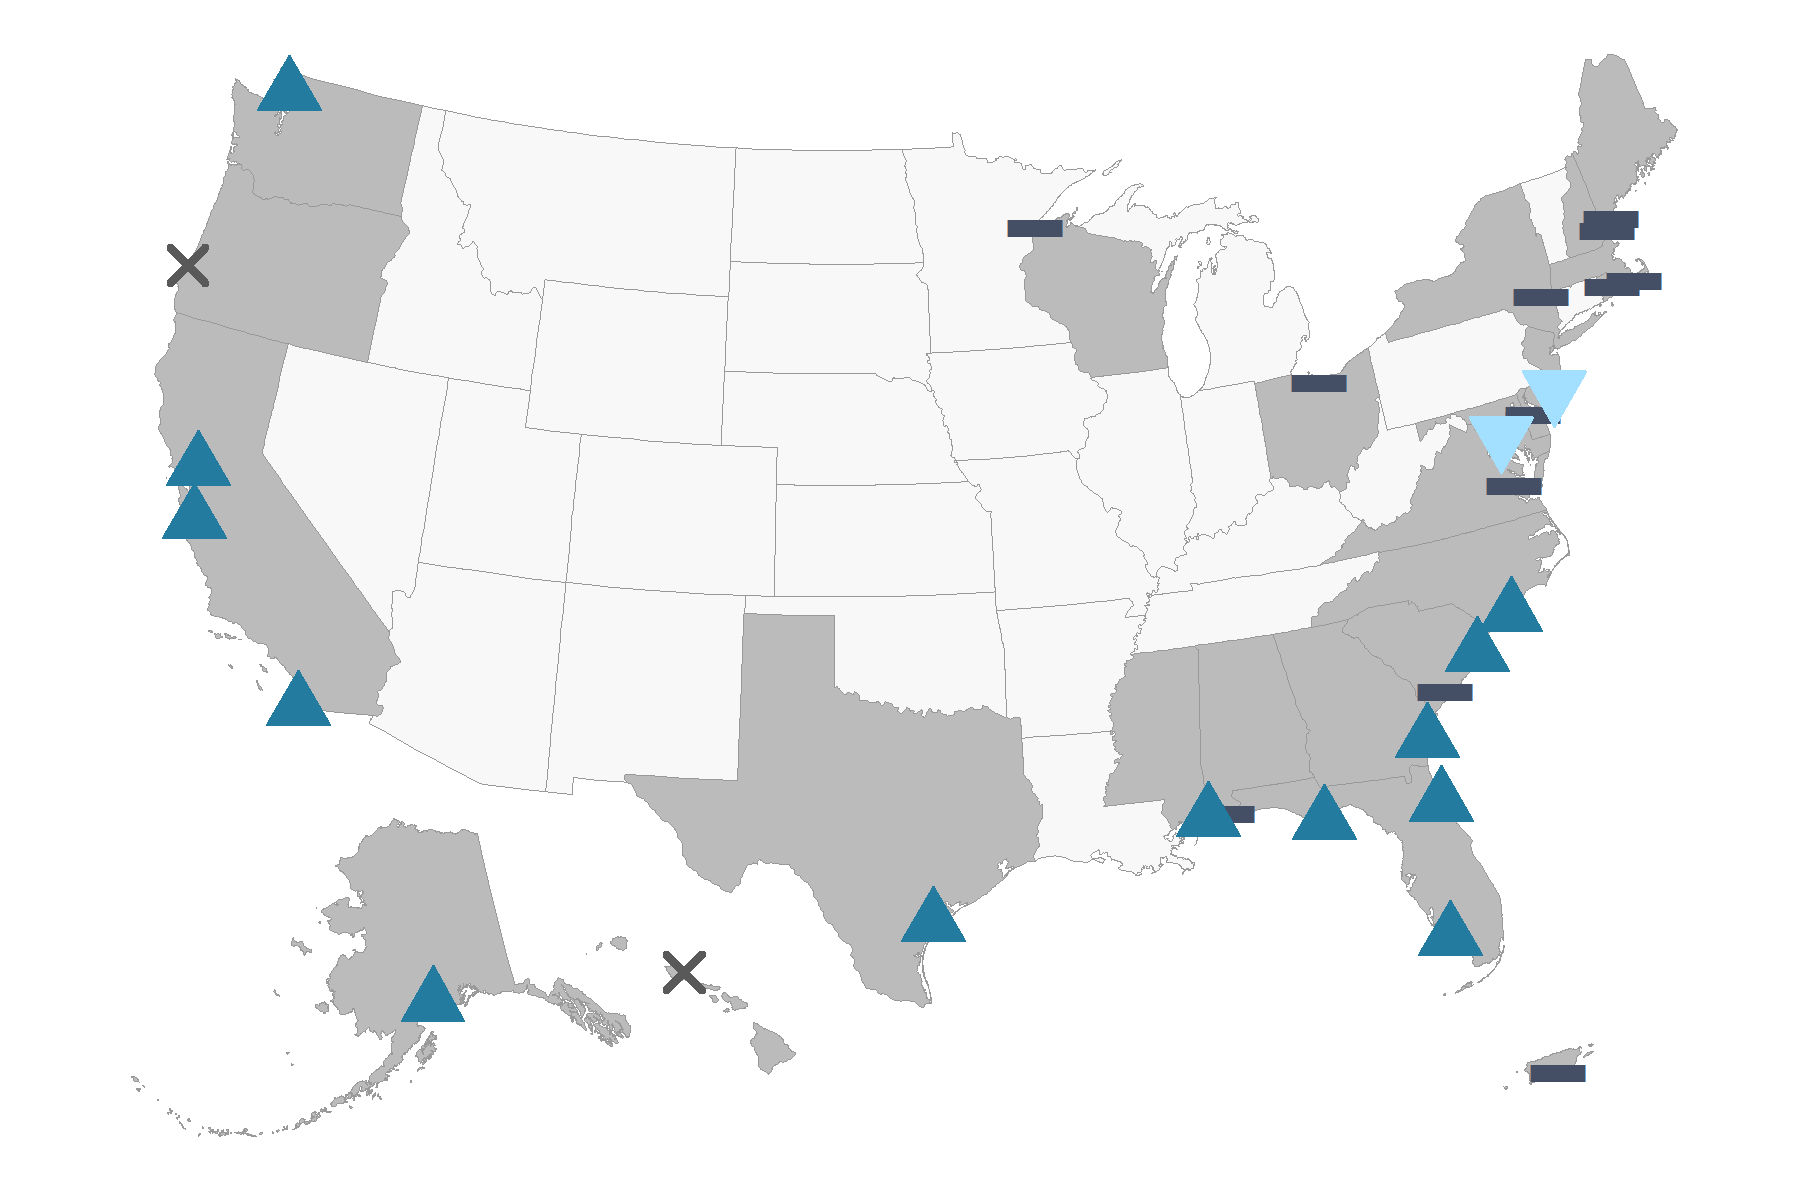
\includegraphics[width=25in]{images/nerrs_map} 

}

\caption{National Estuarine Research Reserve locations in the US.}\label{fig:nerrUS}
\end{figure}

Within a particular NERR there may be several sampling locations (Fig.
\ref{fig:waquoit}), so the next decision would be whether to include
many stations or a subset of stations representing certain conditions
(or having the longest time series).

\begin{figure}

{\centering 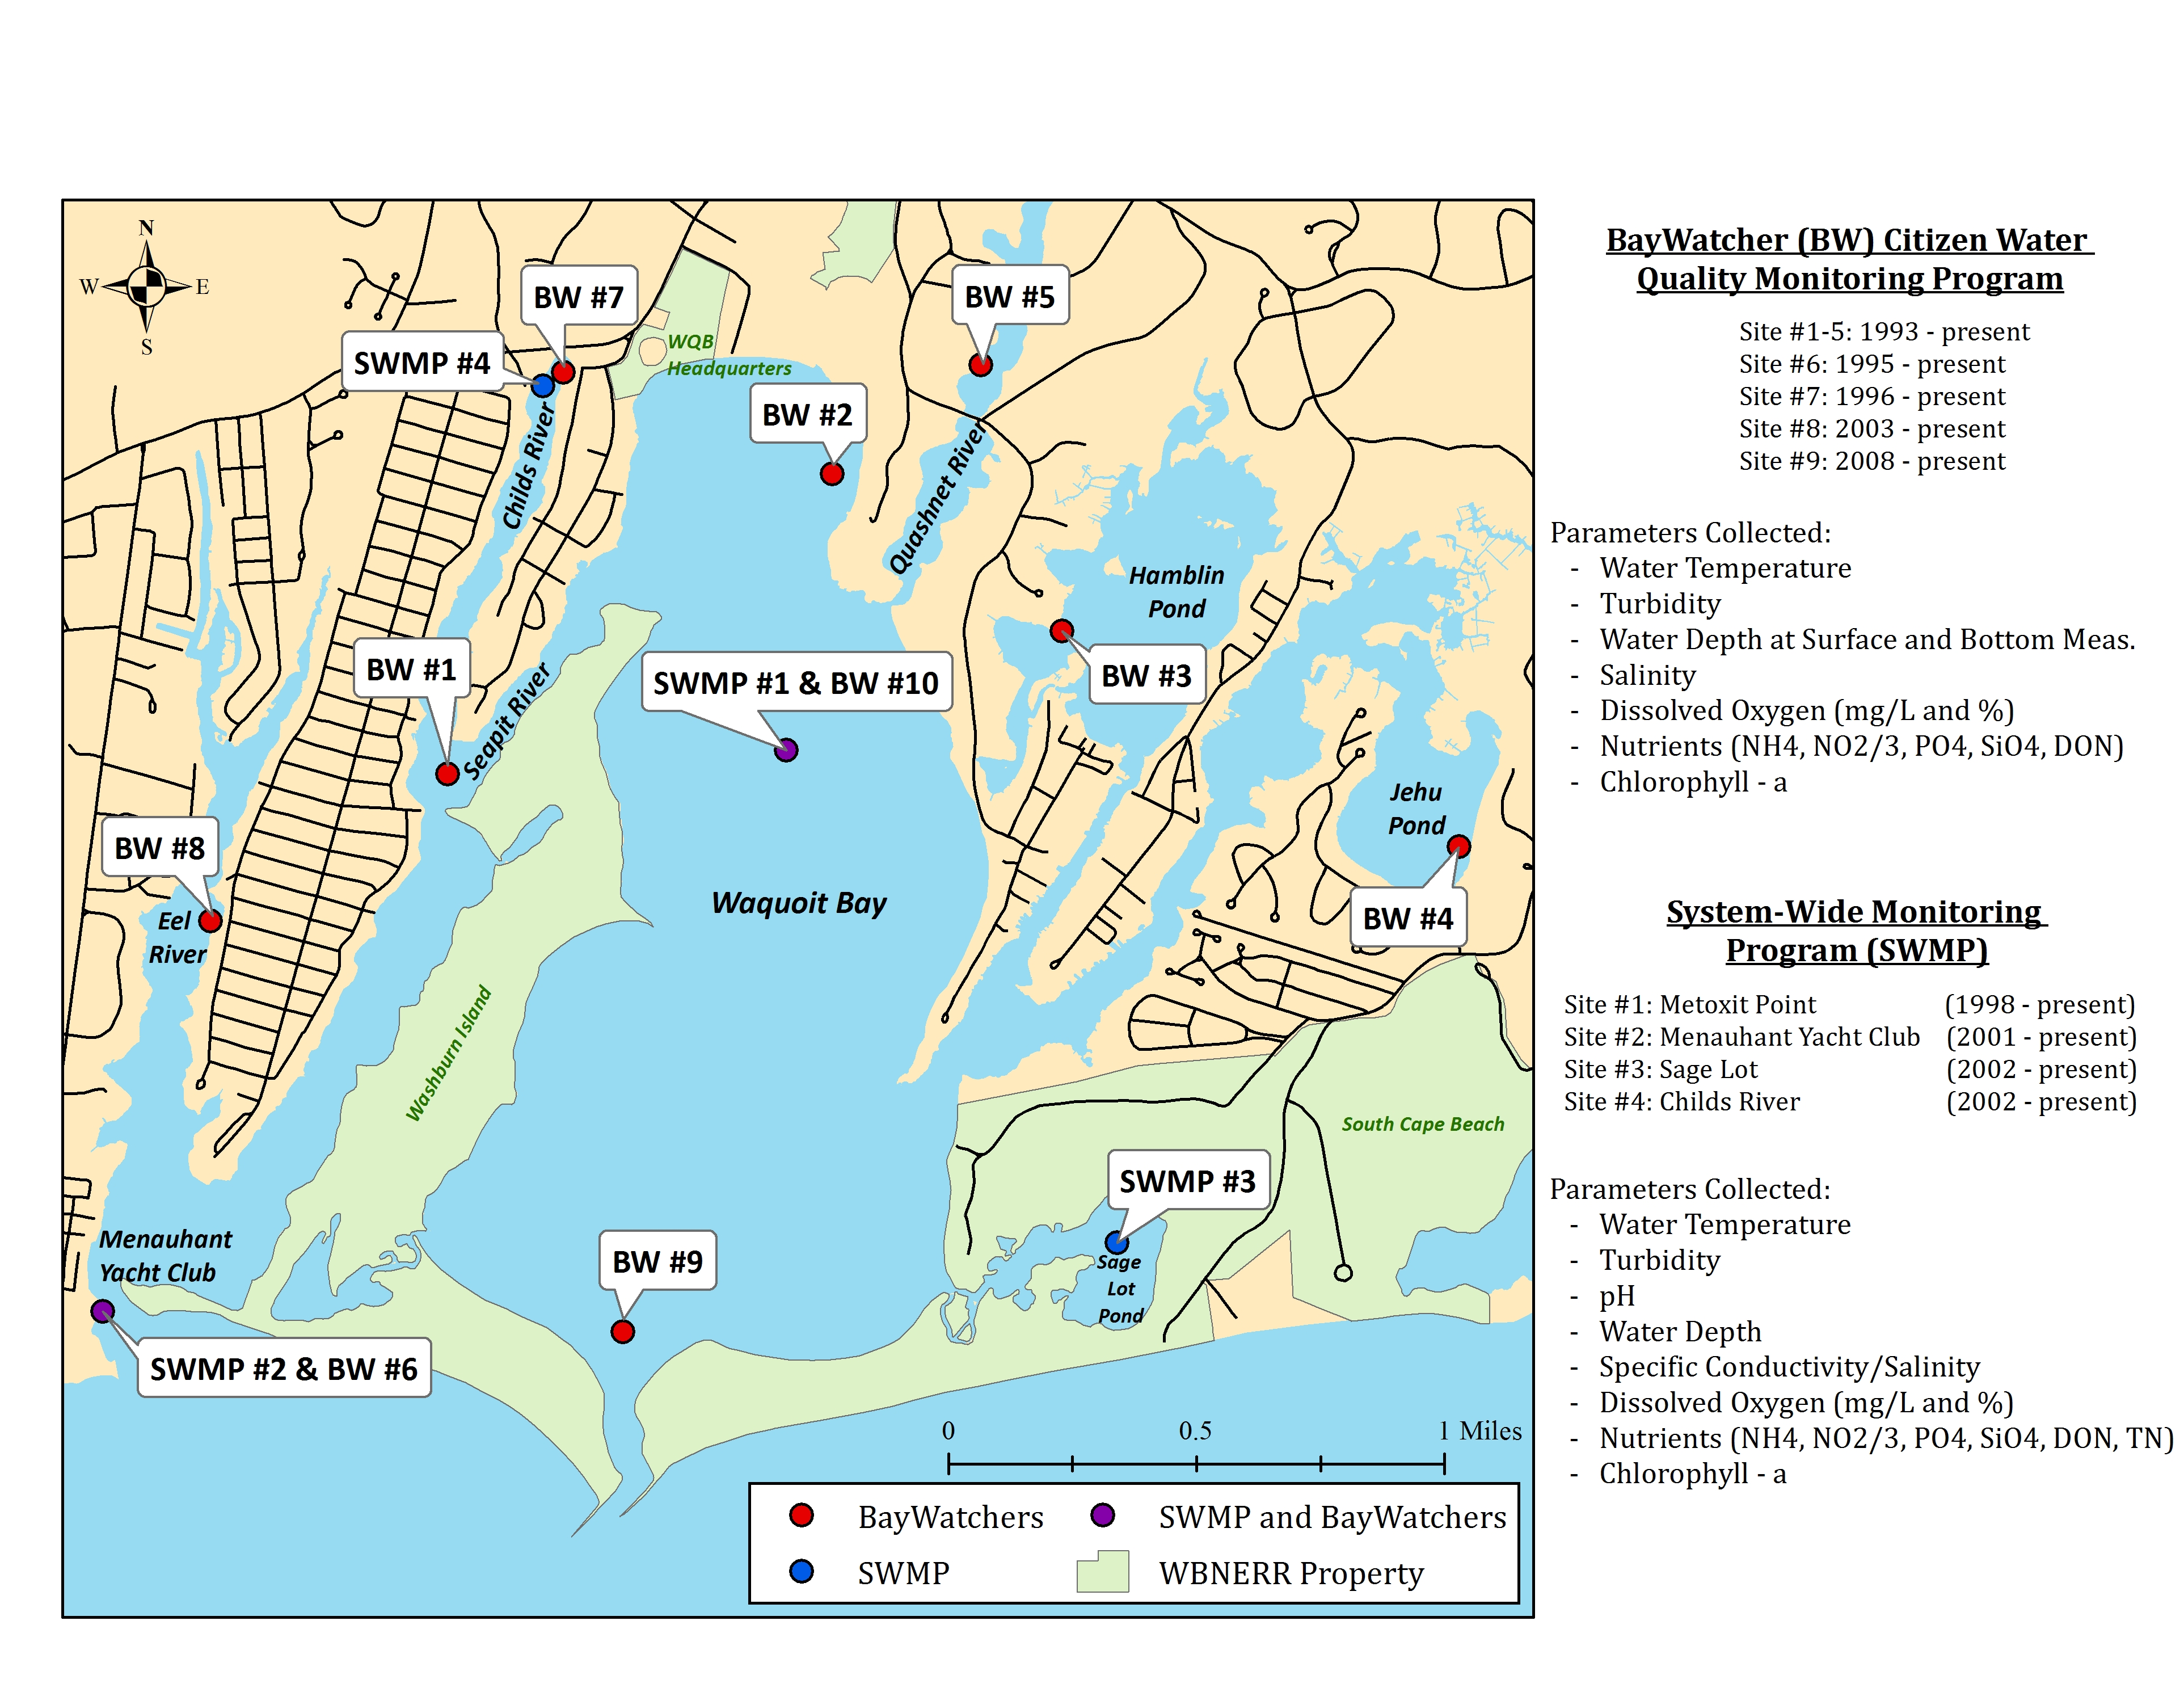
\includegraphics[width=0.95\linewidth]{images/Waquoit_Map} 

}

\caption{Waquit Bay National Estuarine Research Reserve map with sampling locations.}\label{fig:waquoit}
\end{figure}

At each station several types of data are collected, so the next
decision is which type of information is most useful for the Councils?
For example, multiple indicators could contribute to water quality
overall in an area, and could be annual or seasonal (Fig.
\ref{fig:nerr-mult}), or a single indicator of nutrient input could be
of interest across multiple areas (Fig. \ref{fig:nerr-DIN}).

\begin{figure}

{\centering 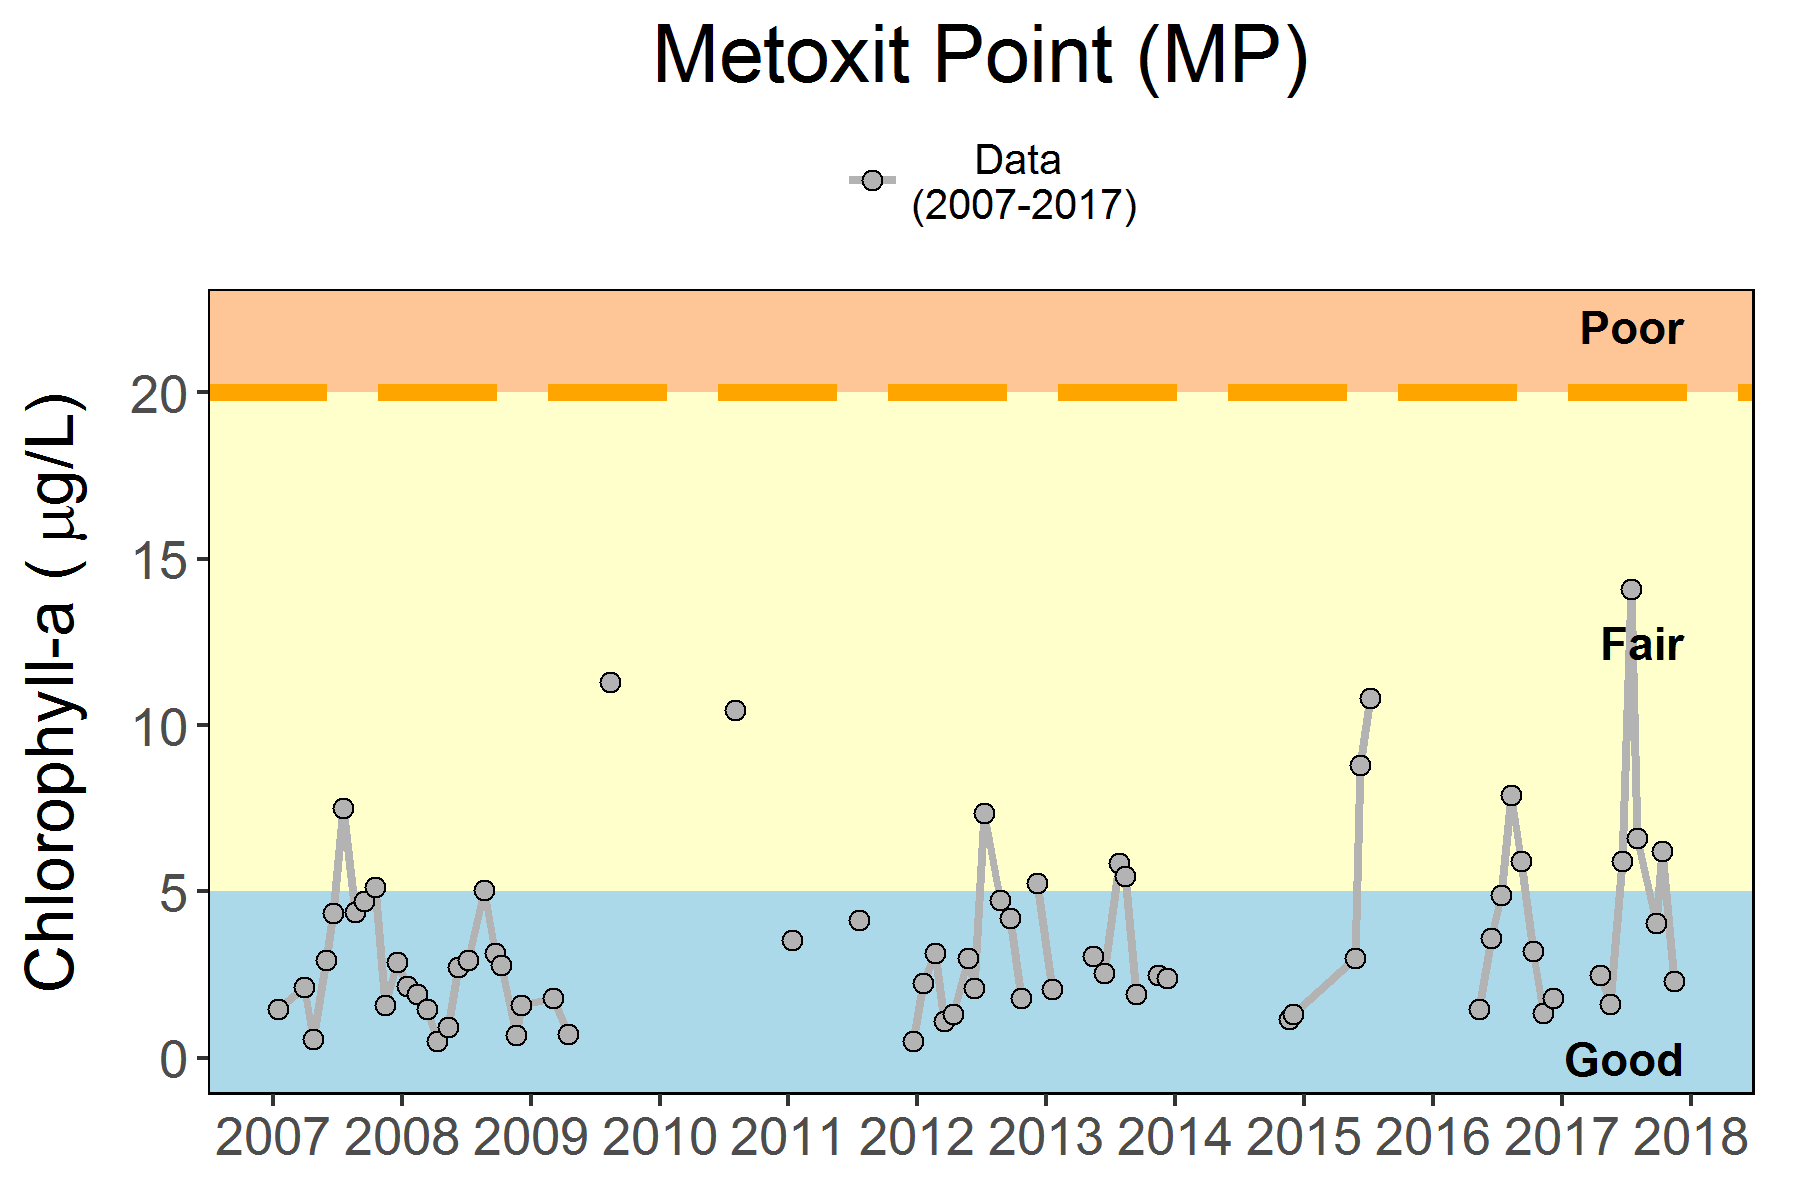
\includegraphics[width=0.49\linewidth]{images/NERRs_Chla} \includegraphics[width=0.49\linewidth]{images/NERRs_DO} 

}

\caption{Multiple water quality attributes.}\label{fig:nerr-mult}
\end{figure}

\begin{figure}

{\centering 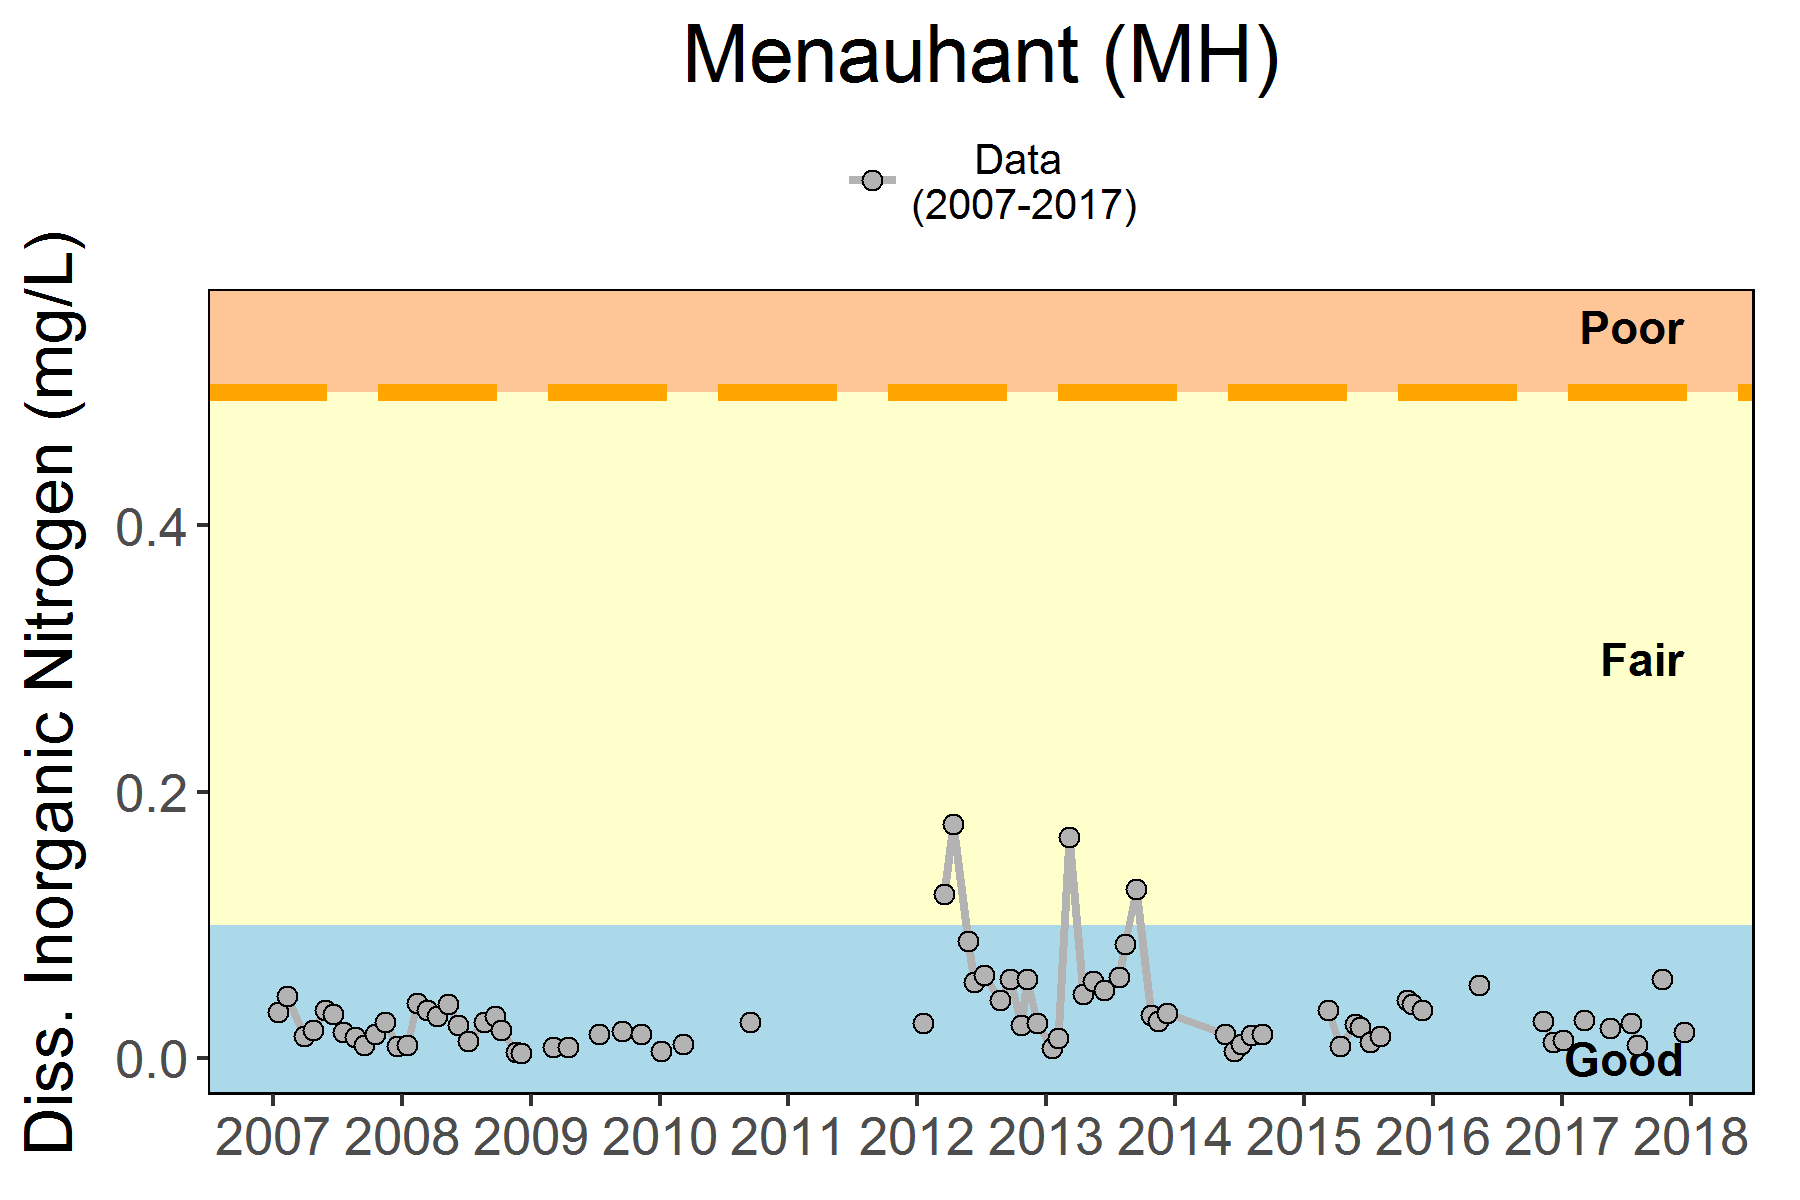
\includegraphics[width=0.49\linewidth]{images/NERRs_MH_DIN} 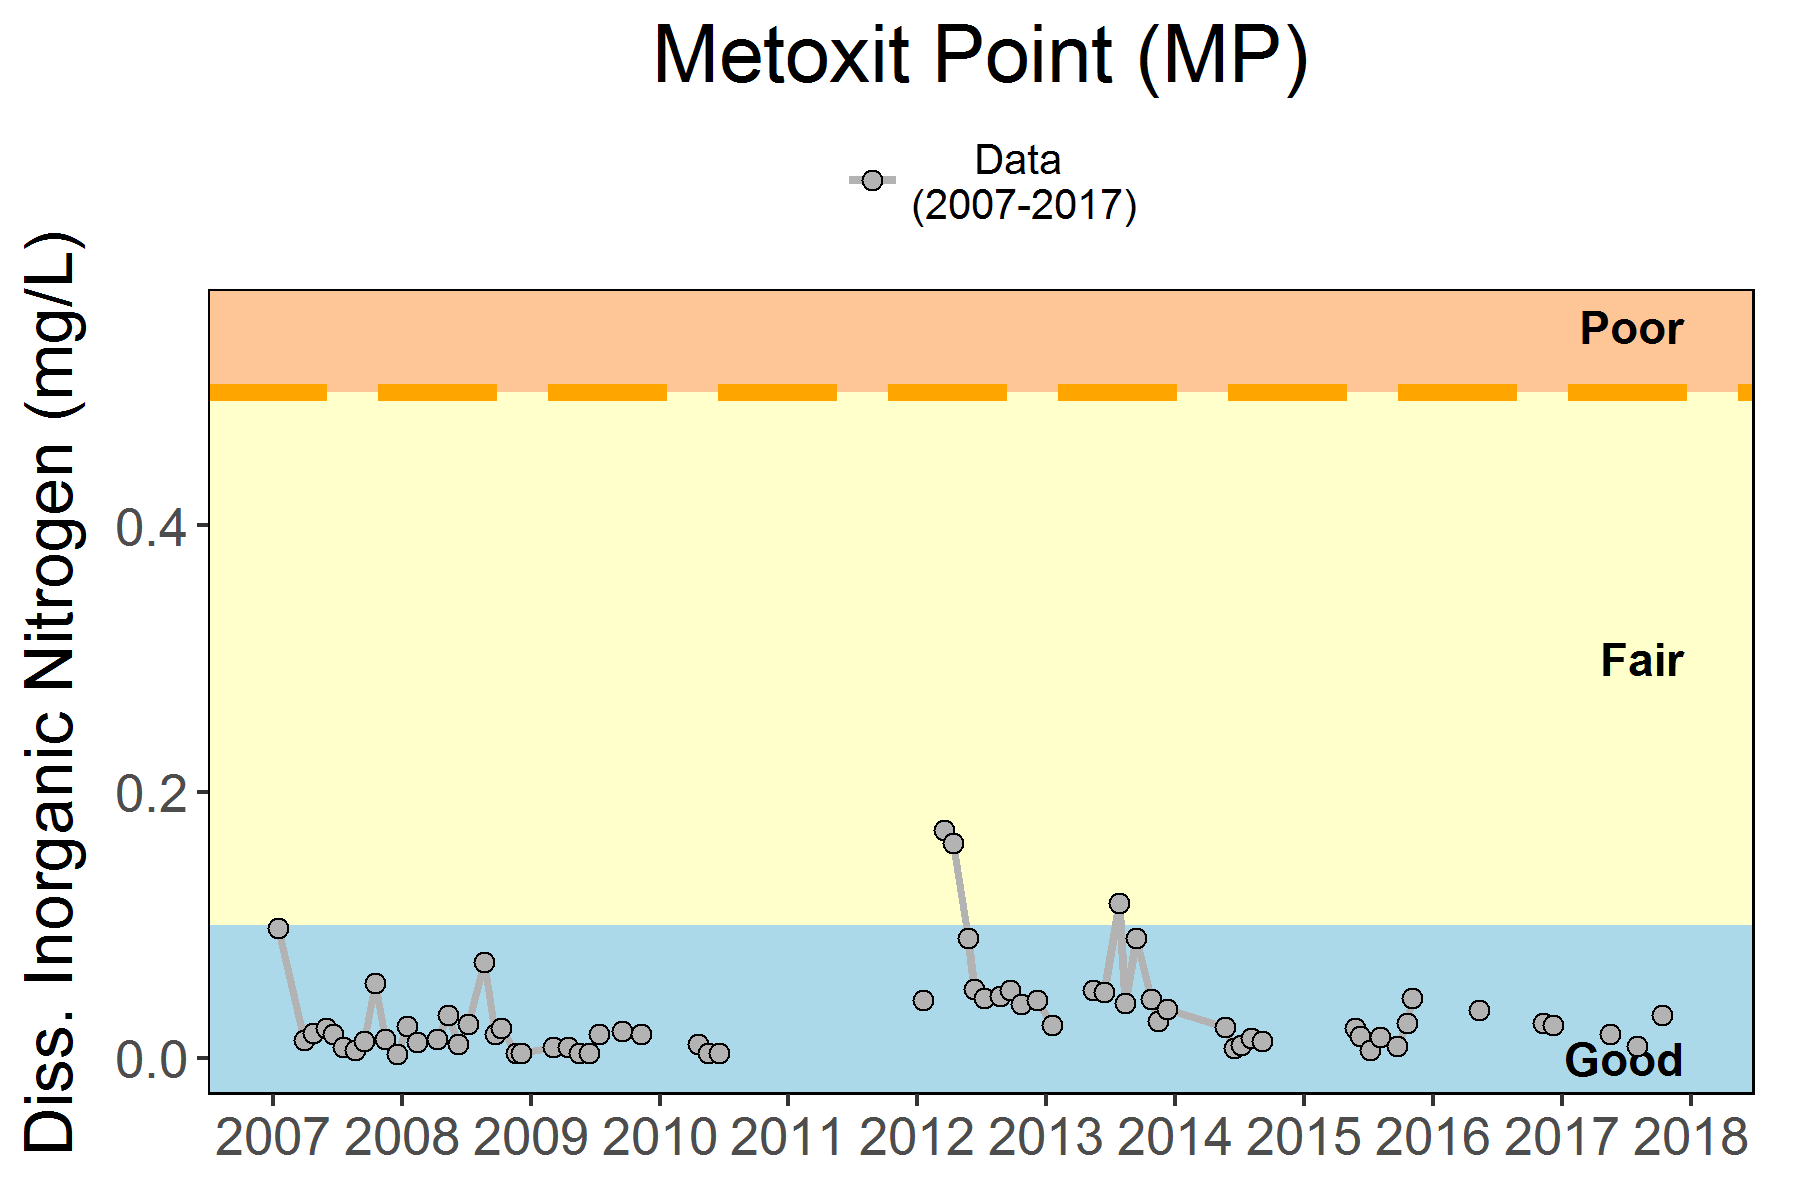
\includegraphics[width=0.49\linewidth]{images/NERRs_MP_DIN} 

}

\caption{Dissolved Inorganic Nitrogen (DIN) in two locations.}\label{fig:nerr-DIN}
\end{figure}

Finally, thresholds for water quality would need to be reviewed (Fig.
\ref{fig:nerr-DIN}). Several exist and could be used by the Council
depending on the ultimate goal for having the indicator.

\hypertarget{section-13}{%
\subsection{14}\label{section-13}}

The NEFMC asked for more linkages between environmental and social and
economic indicators in the SOE. Two new indicators and the research
spotlight linking environmental indicators, fish condition, and fishery
economic indicators highlighted under point 5 address this request. The
first new indicator places commercial fishery landings in the context of
ecosystem produtivity by calculating the primary production required to
support landings; it is described in detail below. The second new
indicator calculates the probability of occupancy of wind lease areas
based on habitat modeling; it is described in detail in point 15.

\hypertarget{primary-production-required-ppr}{%
\subsubsection{Primary production required
(PPR)}\label{primary-production-required-ppr}}

This indicator is included in both SOEs (p.~MAFMC and p.~NEFMC). It is
defined as

\[PPR_t = \sum_{i=1}^{n_t}  \left(\frac{landings_{t,i}}{9}\right) \left(\frac{1}{TE}\right)^{TL_i-1}\]
where \(n_t\) = number of species in time \(t\), \(landings_{t,i}\) =
landings of species \(i\) in time \(t\), \(TL_i\) is the trophic level
of species \(i\), \(TE\) = Trophic efficiency. The PPR estimate assumes
a 9:1 ratio for the conversion of wet weight to carbon and a constant
transfer efficiency per trophic level.

We have explored the index in the following ways. Using:

\begin{itemize}
\item
  \emph{A global transfer efficiency of 15\% for all species.}

  This probably needs some refinement and can/should be adapted based on
  previous studies. One adaptation would be to use a different transfer
  efficienct for the first level. eg.
  \(\left( \frac{1}{TE_1}\right) \left(\frac{1}{TE_2}\right)^{TL_i-2}\).
  Whatever choices are made, the sensitivity of the index to such
  changes should be examined.
\item
  \emph{Primary production not lagged with landings.}

  This is probably not realistic. You wouldn't expect to see changes in
  the landing the same year as changes in primary production. This needs
  to be explored, either using specific lags in time (which may prove
  problematic since species lower on the food chain will be effected by
  shorter lags in time versus species higher up the chain) or by
  adopting some weighted scheme.
\item
  \emph{A threshold of 80\% for landings.}

  It would be a good idea to explore the sensitivity of the index for
  other threshold levels. Of course the higher the threshold used would
  imply that less common species will then contribute to the index.
\item
  \emph{Combined vertebrates and invertebrates.}

  The landings in some of the EPUs are dominated by invertebrates
  (Lobster, Clams) which may play a significant part in driving this
  index. Creating two additional indices, one for vertebrates and one
  for invertebrates may be an interesting avenue. This will of course
  imply the inclusion of many other lesser caught species into the
  index. It will also involve partitioning the landings into vertebrates
  and invertebrates.
\end{itemize}

\emph{Other comments}

\begin{itemize}
\item
  Some classifications in the commercial fisheries database are not at
  the species level. Some are Genus, Family or even higher orders, some
  are just general unclassified. eg. (DOGFISH, UNC, FLATFISH,
  Argentinidae). Most of these cases are associated with lower landings.
  However if we increase the threshold and/or split landings into
  vertebrates and invertebrates we will encounter more of these
  classifications. They will need to be assigned a trophic level which
  may cause complications and/ or subjective decision making.
\item
  It is possible for species to drop out of the top x\% of the landings
  and be replaced by other species with a similar trophic level and the
  index will be somewhat insensitive to this (Fig.
  \ref{fig:ppr-species}). The mean trophic level would also be
  insensitive to such changes. This may or may not be of concern, but it
  may be worth looking into how often this occurs.
\end{itemize}

\begin{figure}

{\centering 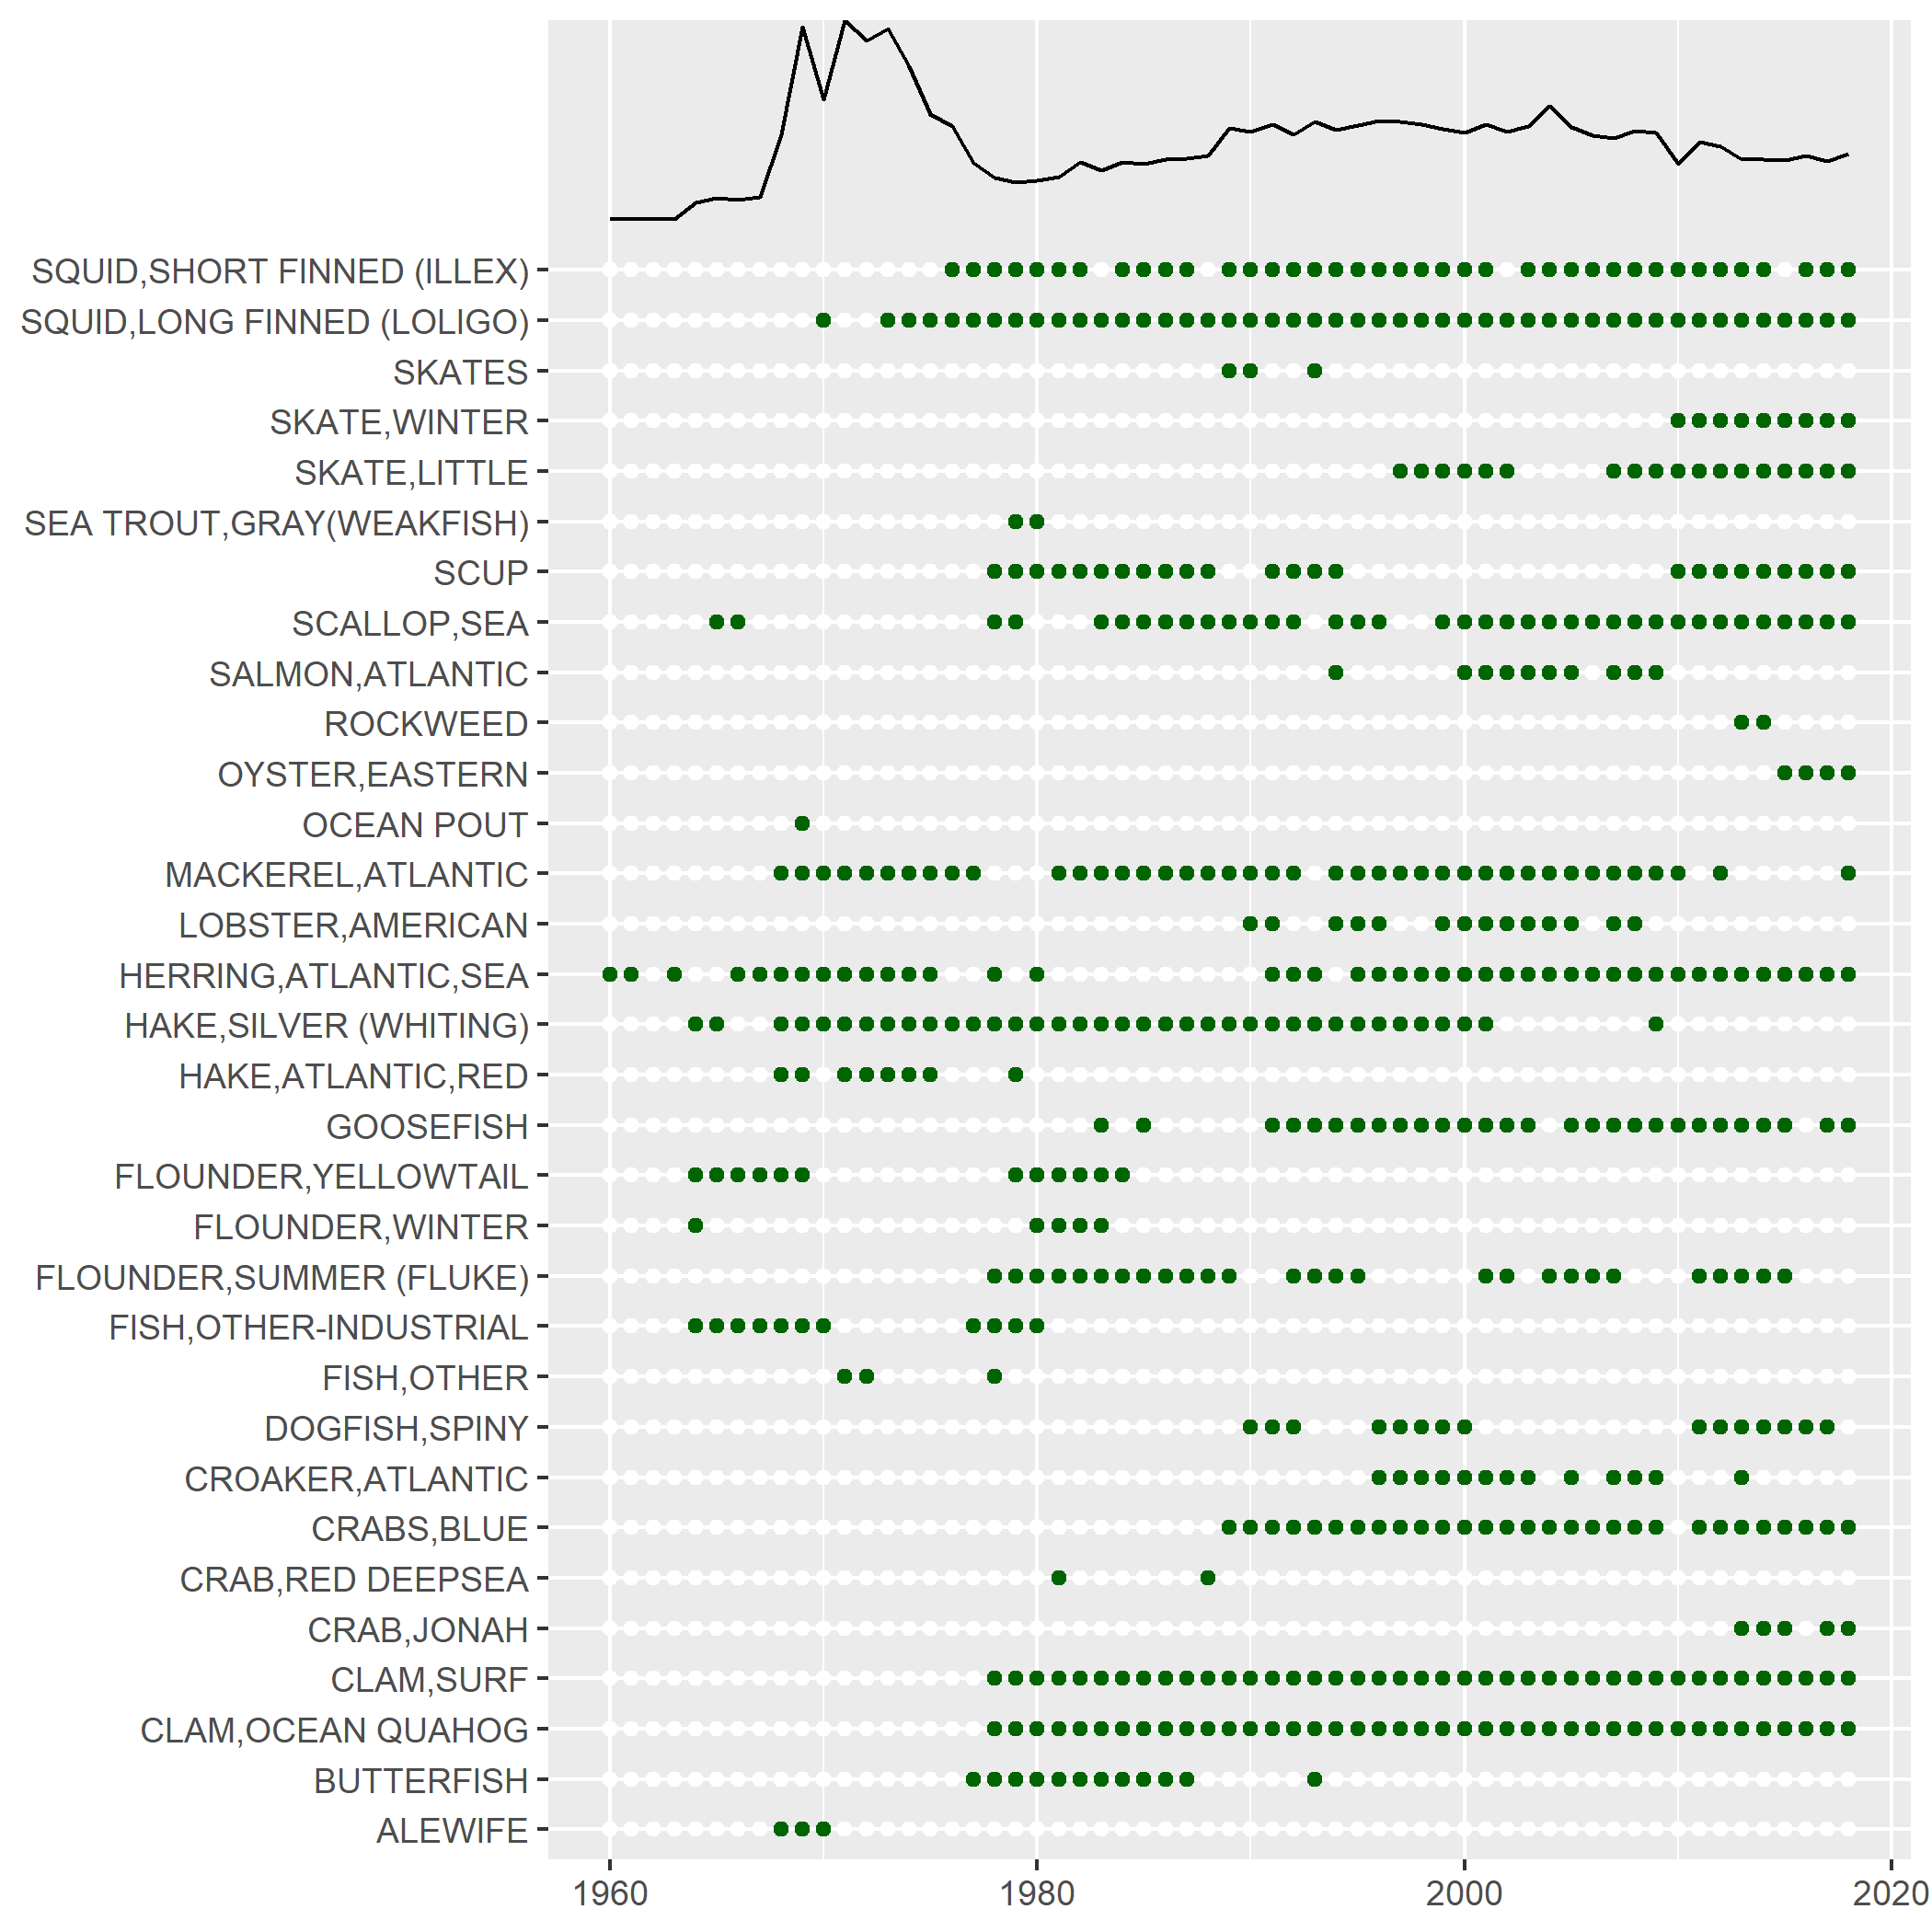
\includegraphics[width=0.32\linewidth]{images/composition-MAB-0_80} 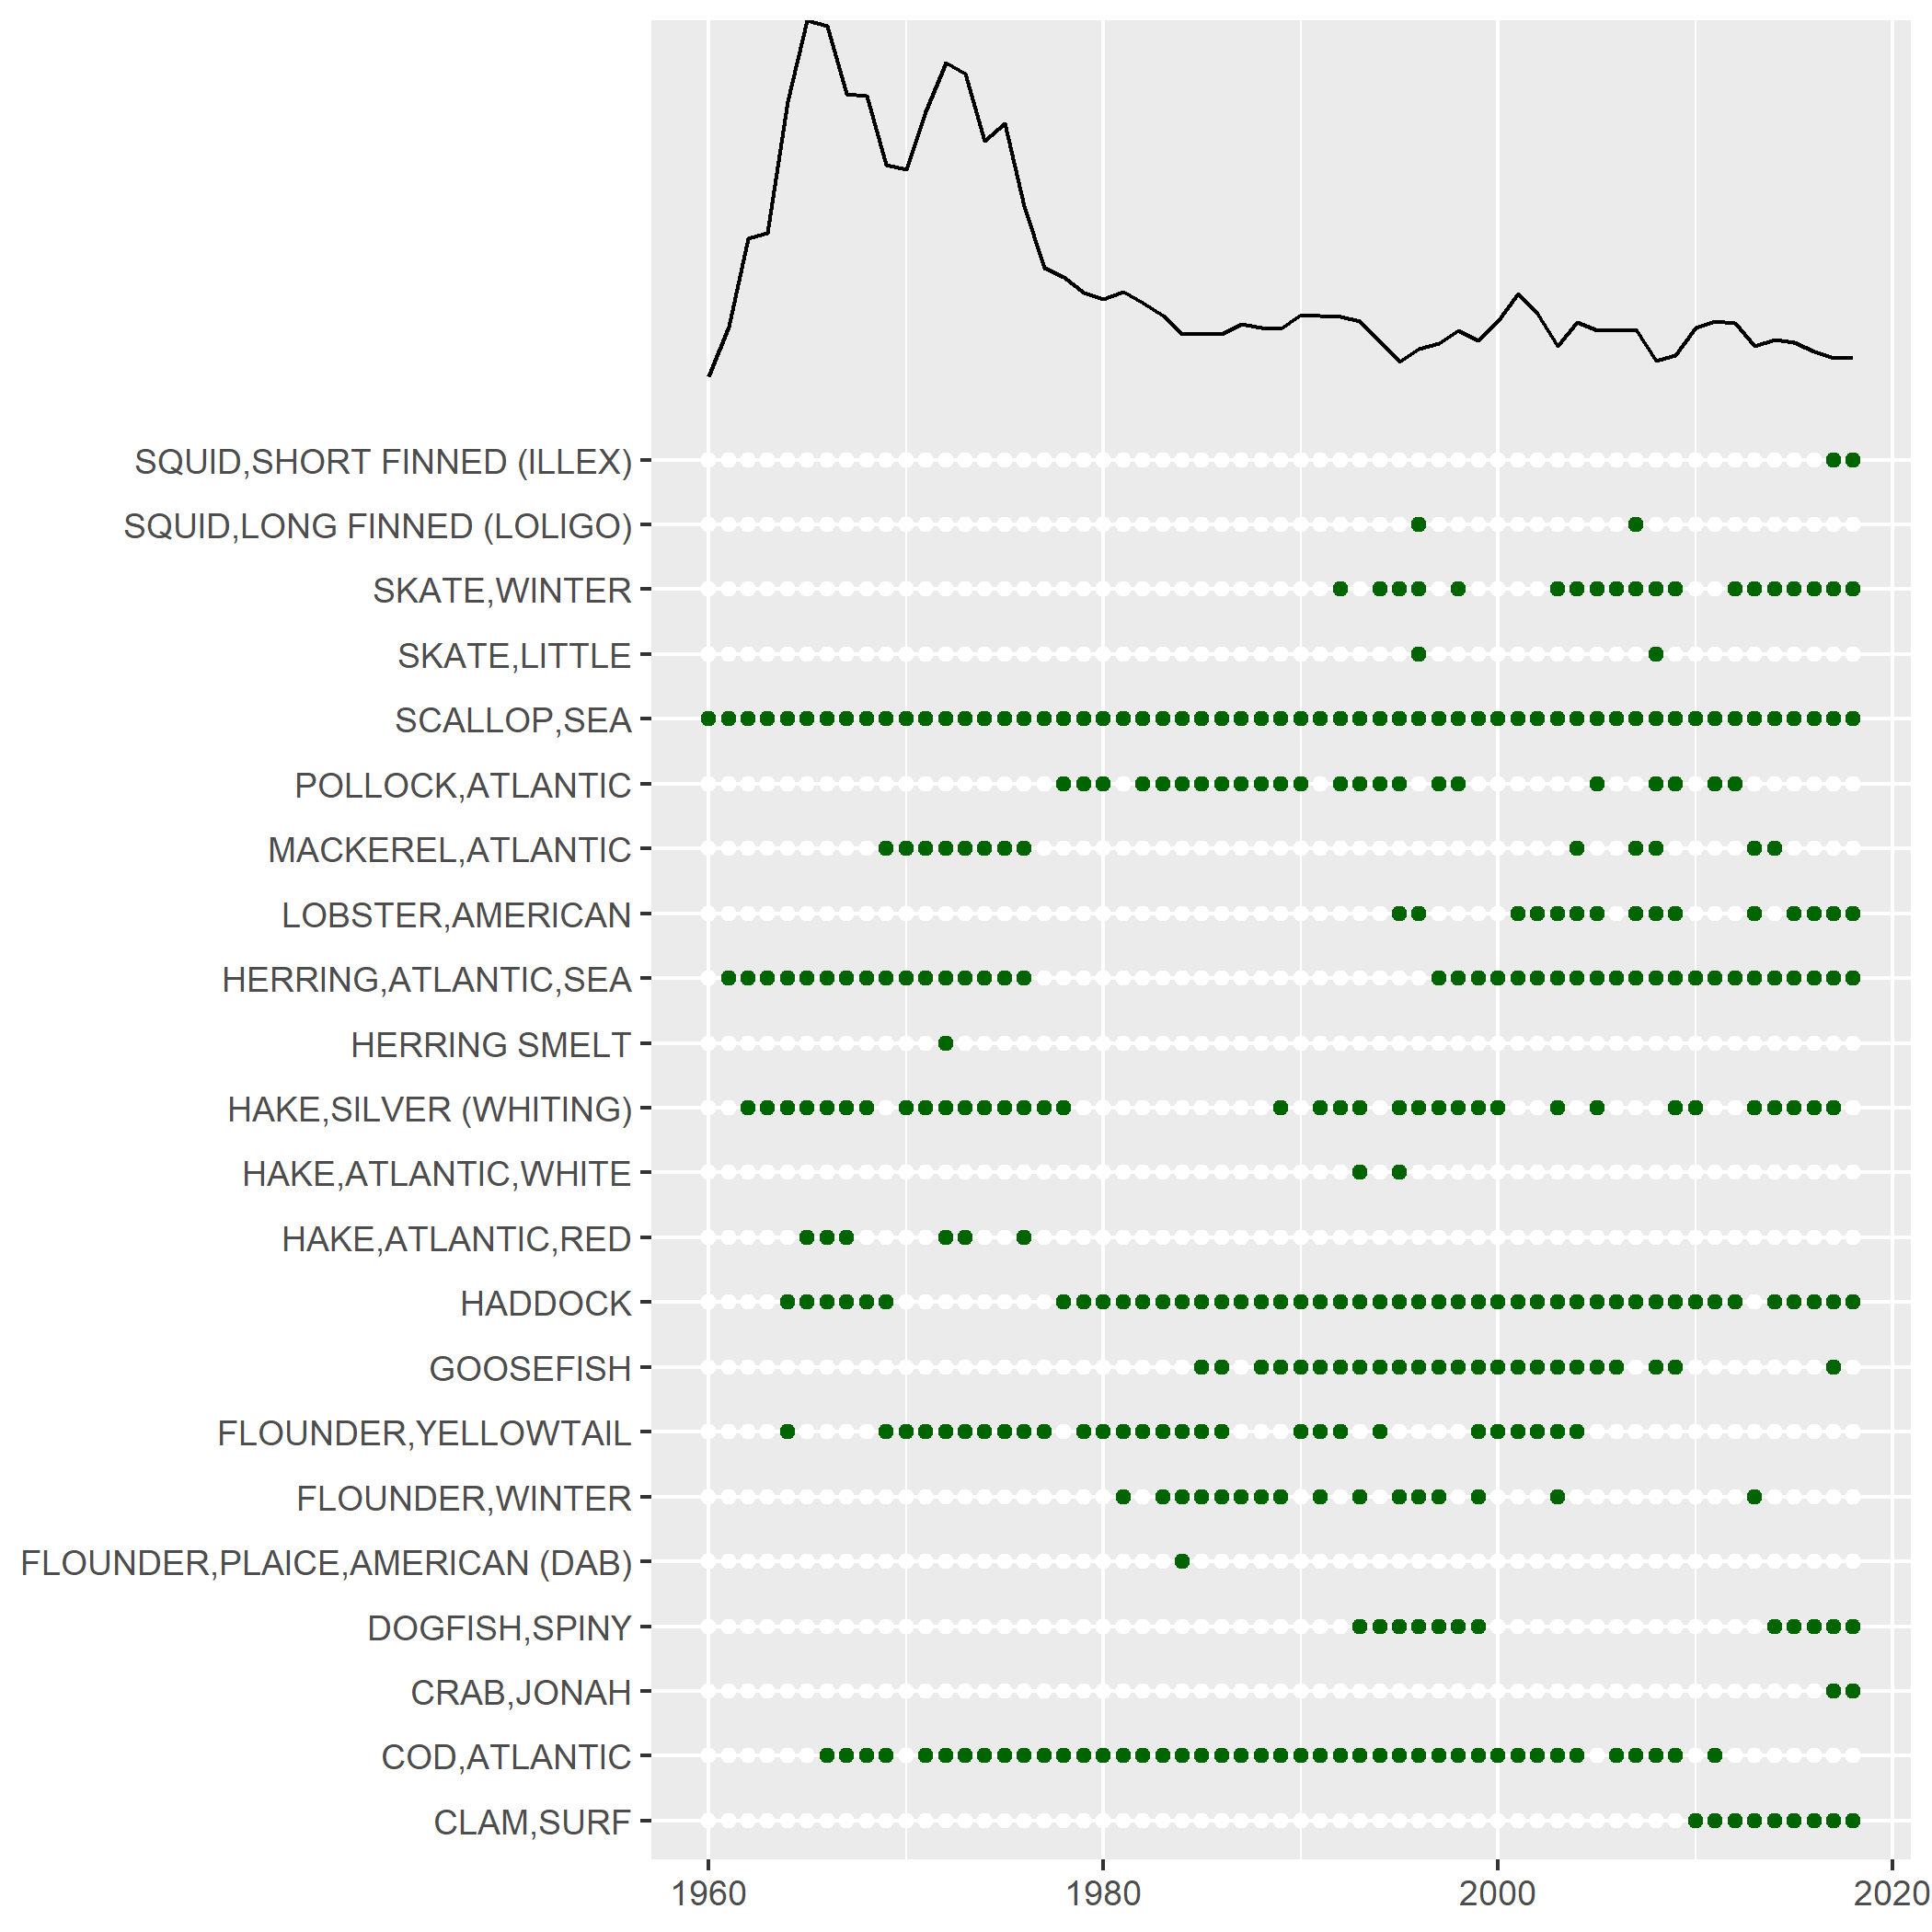
\includegraphics[width=0.32\linewidth]{images/composition-GB-0_80} 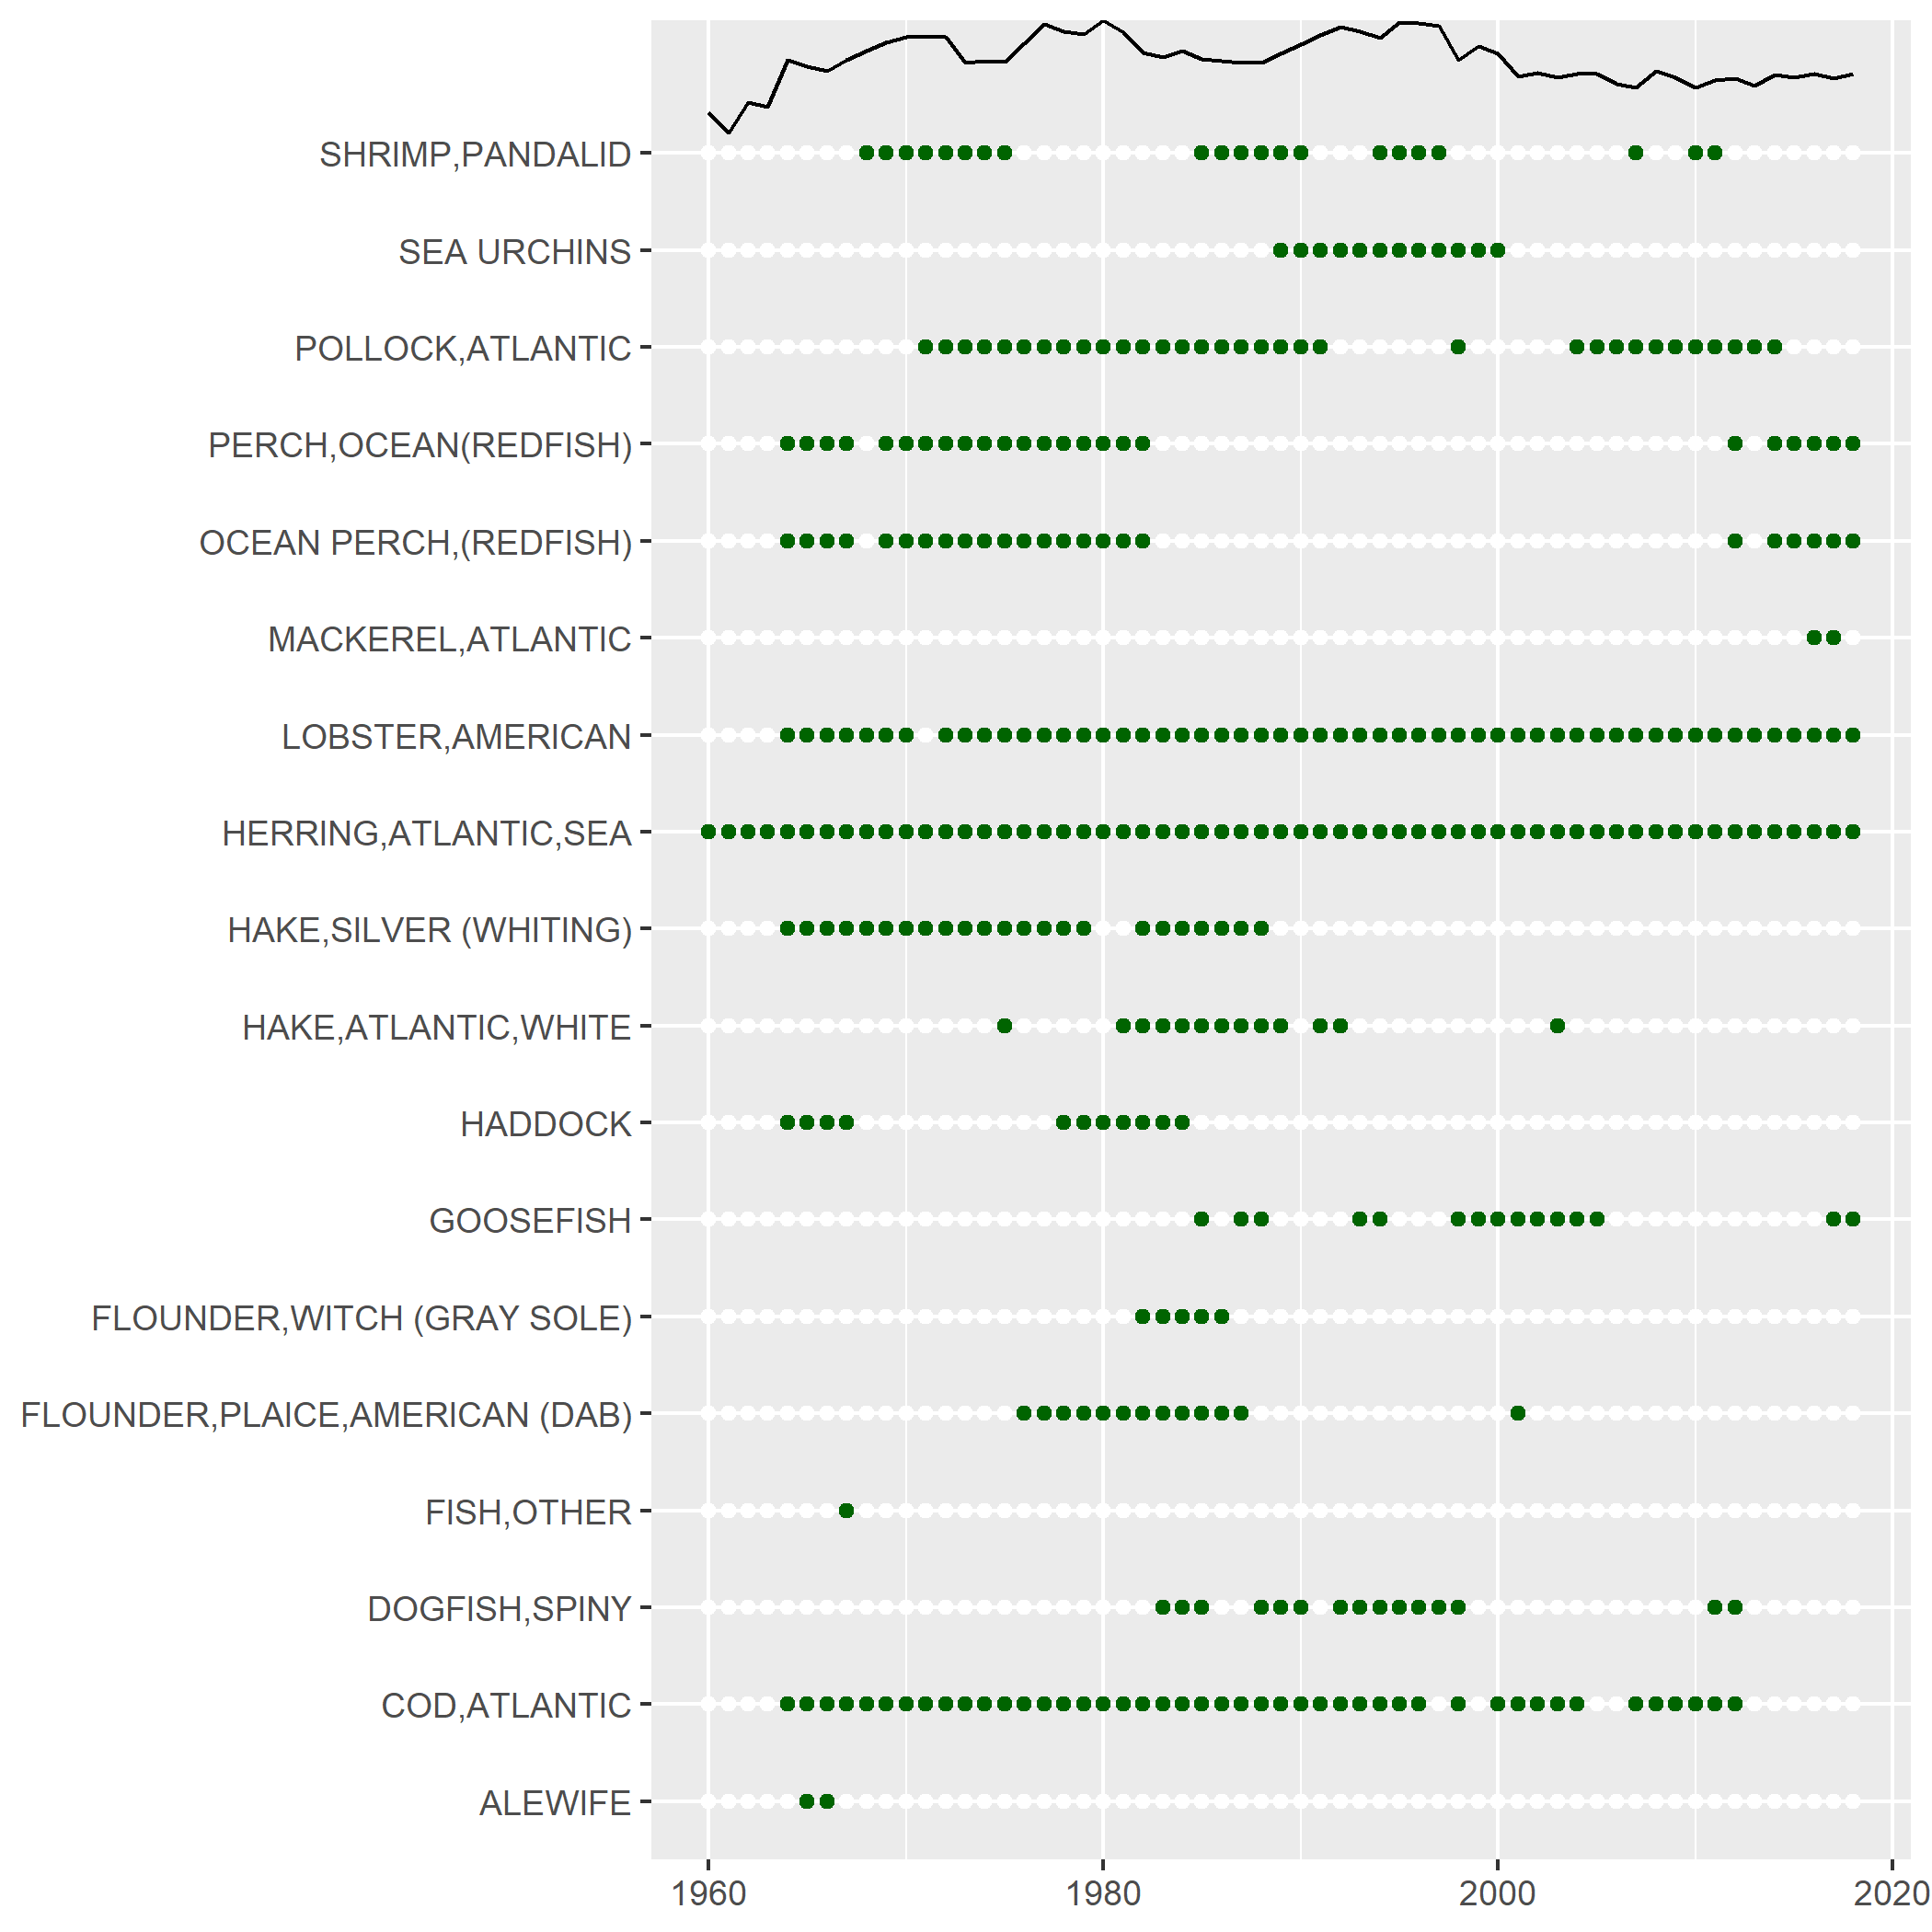
\includegraphics[width=0.32\linewidth]{images/composition-GOM-0_80} 

}

\caption{Species included in 80\% of landings for each year in the Mid-Atlantic Bight (left), Georges Bank (center), and Gulf of Maine (right).}\label{fig:ppr-species}
\end{figure}

We welome feedback for approaches to refine this indicator.

\hypertarget{section-14}{%
\subsection{15}\label{section-14}}

The MAFMC requested an index of quantitative overlap of wind energy
lease areas and fisheries, in particular to update the EAFM risk
assessment (Other ocean uses risk element). A list of species with the
highest probability of occupancy in the current and proposed wind lease
areas based on habitat modeling is included in both SOEs (p.~MAFMC and
p.~NEFMC). This indicator can be refined to meet the needs of both
Councils. In future reports we plan to include the overlap of current
fisheries with wind lease areas as well.

\hypertarget{section-15}{%
\subsection{16}\label{section-15}}

The NE SSC asked that we include links to NMFS Social Science indicator
websites. These links have been included in both reports (p.~MAFMC and
p.~NEFMC).

\hypertarget{section-16}{%
\subsection{17}\label{section-16}}

The MAFMC asked for indicators of management complexity for use in the
EAFM risk assessment. An NEFSC summer student started work on this in
2018, but we have lacked capacity to finish the project since then. If
resources allow we will continue the project, and guidance for further
indicator developmet is welcome.

\hypertarget{section-17}{%
\subsection{18}\label{section-17}}

The MAFMC asked that South Atlantic Council-managed species be
represented in recreational catch diversity indices. This has been done
and the updated indicator is included in both SOE reports (p.~MAFMC and
p.~NEFMC).

In addition, NEFSC survey data was analyzed to determine if South
Atlantic Council managed species have become more common in the survey
over time. This indicator has also been included in both SOE reports
(p.~MAFMC and p.~NEFMC).

\hypertarget{section-18}{%
\subsection{19}\label{section-18}}

The NEFMC requested that social elements from the overview conceptual
model shown in presentations be added to the New England conceptual
model included in the printed SOE report. While this would be a useful
update, all of the previous conceptual models have been replaced by
different summary visualizations requested by the Councils (see points 1
and 2).

\hypertarget{section-19}{%
\subsection{20}\label{section-19}}

Both Councils were interested in indicators related to fish diet data.
For example, average weight of diet components by feeding group, and
mean stomach weight across feeding guilds were mentioned. We initiated
exploratory analysis of diet information this year, and present examples
of the types of information available to seek feedback on how the
Counicls would like indicators developed further.

On NEFSC surveys, most stomach estimates are taken as a volume measure,
but there is a standard conversion included in the diet database that
gives an approximate stomach weight. This estimated stomach weight was
used to calculate stomach fullness (a proportion from empty = 0 to full
= 1). Stomach fullness may be a better measure than absolute stomach
weight if combining across species into a feeding guild, otherwise big
animals with heavier stomachs will dominate the index. Here, stomach
fullness was expressed as an annual anomaly for each species in each
region. This shows which species have adequate data for inclusion in a
time series, and suggests there are not obvious common stomach fullness
anomalies across species. We welcome suggestions to clarify methods and
objectives for fish stomach data indicators.

\begin{figure}

{\centering \includegraphics{2020RespMemoBody_files/figure-latex/ma-stomachs-1} 

}

\caption{Stomach fullness anomaly in the Mid-Atlantic Bight.}\label{fig:ma-stomachs}
\end{figure}

\begin{figure}

{\centering \includegraphics{2020RespMemoBody_files/figure-latex/ne-stomachs-1} 

}

\caption{ Stomach Fullness Anomaly in New England.}\label{fig:ne-stomachs1}
\end{figure}
\begin{figure}

{\centering \includegraphics{2020RespMemoBody_files/figure-latex/ne-stomachs-2} 

}

\caption{ Stomach Fullness Anomaly in New England.}\label{fig:ne-stomachs2}
\end{figure}

\hypertarget{section-20}{%
\subsection{21}\label{section-20}}

The NEFMC requested a North Atlantic Right Whale calf production
indicator. This indicator has been added to both SOE reports (p.~MAFMC
and p.~NEFMC).

\hypertarget{section-21}{%
\subsection{22}\label{section-21}}

The NEFMC requested that managed species be distinguished in the report.
Both SOE reports summarize landings as a whole and by Council-managed
species in aggregate (p.~MAFMC and p.~NEFMC). A table listing which
species are managed by which entity is included in each SOE report
(Table 4 in both reports). Status of Council-managed species is reported
in each SOE (p.~MAFMC and p.~NEFMC) with jointly managed species
indicated.

\hypertarget{section-22}{%
\subsection{23}\label{section-22}}

The MAFMC was interested in estimates of marine mammal consumption.
While there have been no updated reports of total marine mammal
consumption for the US Northeast Shelf ecosystem since 2015
{[}\protect\hyperlink{ref-smith_consumption_2015}{6}{]}, new diet
studies are in progress. We included updated information on seal diets
in both SOE reports (p.~MAFMC and p.~NEFMC). Once completed, these diet
studies combined with mammal population estimates could be used to
update marine mammal consumption estimates.

\hypertarget{section-23}{%
\subsection{24}\label{section-23}}

The MAFMC requested indices of small pelagic abundance. While the SOE
includes survey biomass estimates of planktivores (p.~MAFMC and
p.~NEFMC), we would like to improve on these indices. Combining survey
information using VAST models as described under point 3 may improve
indices for small pelagics, but species not sampled by bottom trawl
surveys remain problematic. We welcome feedback on other sources of
information to address small pelagic abundance.

Forage energy content is another important consideration which may
affect predators as much as fluctuations in abundance. This year we have
included initial information on forage energy content in the SOE reports
(p.~MAFMC and p.~NEFMC) which highlights the potential for seasonal and
interannual variability in energy content. We plan to develop forage
energy content indicators as this time series develops, and welcome
feedback on how best to do so.

\hypertarget{section-24}{%
\subsection{25}\label{section-24}}

The MA SSC was interested in a young of year index from multiple
surveys. We have included the fish productivity index in both SOE
reports (p.~MAFMC and p.~NEFMC), which calculates the number of small
fish per biomass of large fish of the same species from NEFSC surveys.
This index has been reported previously to MAFMC, and intermittently to
NEFMC. We recognize that this is not strictly a young of year index, and
it is from a single survey. We seek guidance from the SSC on how to
refine this index; would a similar index of small fish numbers to large
fish biomass from the NEAMAP survey data be useful? Or would an index of
young of year without biomass of larger fish be more useful? If so, how
would we best combine species or select species for the index? And
should we try to combine surveys or report them separately?

\hypertarget{section-25}{%
\subsection{26}\label{section-25}}

The MAFMC requested information on biomass of sharks, as fishermen had
reported encountering more blacktip, spinner, and sandbar sharks each
summer. We were able to obtain catch data from the Highly Migratory
Species group at NMFS Headquarters for the past 3 years, and the group
is working on assembling a longer time series for future reports. We did
not print the 3 year time series in the SOE reports, but visualizations
are available along with other commercial landings\footnote{\url{https://noaa-edab.github.io/ecodata/human_dimensions}}.
To date, we have been unable to get biomass information on sharks at the
coastwide level. We welcome suggestions for sources of this information.

\hypertarget{section-26}{%
\subsection{27}\label{section-26}}

The NE SSC requested a species diversity metric based on NEFSC trawl
survey data. We have included such a metric in past reports (2017), but
were concerned that apparent differences in diversity prior to and after
2008 may be driven by differences in survey vessels. While
species-specific cpue and sizes have calibration coefficents between
survey vessels, the number of species captured by the vessels has no
known calibration coefficient.

We could calculate diversity indices for Albatross and Bigelow years
separately to avoid this issue, and will do so if the Councils would
find these separate indices useful.

\hypertarget{section-27}{%
\subsection{28}\label{section-27}}

The MAFMC requested work towards an ecosystem-level risk score. This
system level score could augment information on individual risk elements
already included in the MAFMC EAFM risk assessment, which is updated
annually. Multiple indicators could be combined to form an integrated
risk score (as discussed by the MAFMC Ecosystem and Ocean Planning
Committee when evaluting this EAFM risk assessment), and many integrated
scores have been suggested in the scientific literature. We seek further
guidance on how best to develop an integrated ecosystem risk score for
the MAFMC and NEFMC.

In the meantime, the primary production required to support landings
introduced in this year's SOEs (p.~MAFMC and p.~NEFMC) may contribute to
an overall ecosystem risk score. While there is no established threshold
for primary production required, fisheries would likely pose higher
ecosystem risk if they require very high proportions of primary
production. We welcome comments and suggestions from the Councils to
continue this work.

Similarly, the new SOE marine heat wave indicator (p.~MAFMC and
p.~NEFMC) may contribute to an overall ecosystem risk score from a
climate/environmental perspective, as it measures the frequency of
extreme temperature conditions in each EPU which pose risks to ecolgical
and fishing communities. This could be integrated with existing climate
vulnerability information and/or other report indicators to assess risk.
Ultimately, the Council's objectives for this risk score will determine
the components used.

\hypertarget{section-28}{%
\subsection{29}\label{section-28}}

Both Councils have been interested in ecosystem-level thresholds and
determining where indicators reach inflection points, suggesting changes
in trends of concern. The SOEs include statistical analysis to determine
where indicators have significant increasing or decreasing trends.
However, based on a recent simulation analysis, we are confident in
trend assessment only for time series of 30 years or more
{[}\protect\hyperlink{ref-hardison_simulation_2019}{7}{]}.

Some SOE indicators, such as the new marine heat wave cumulative
intensity indicator in the Gulf of Maine (p.~NEFMC) have both
significant trends and visually obvious shifts that could reflect a
change in state for that indicator, which could be confirmed with
further statistical analysis. Work is ongoing to determine statistically
where shifts or changepoints across multiple indicators have ocurred,
but was not ready for inclusion in this year's reports. We welcome
comments and guidance from the Councils on the types of analysis that
would be most useful: changepoints for individual indicators, or across
many indicators, or both?

\hypertarget{references}{%
\section*{References}\label{references}}
\addcontentsline{toc}{section}{References}

\hypertarget{refs}{}
\leavevmode\hypertarget{ref-zador_ecosystem_2016}{}%
1. Zador SG, Holsman KK, Aydin KY, Gaichas SK. Ecosystem considerations
in Alaska: The value of qualitative assessments. ICES Journal of Marine
Science: Journal du Conseil. 2016; fsw144.
doi:\href{https://doi.org/10.1093/icesjms/fsw144}{10.1093/icesjms/fsw144}

\leavevmode\hypertarget{ref-thorson_guidance_2019}{}%
2. Thorson JT. Guidance for decisions using the Vector Autoregressive
Spatio-Temporal (VAST) package in stock, ecosystem, habitat and climate
assessments. Fisheries Research. 2019;210: 143--161.
doi:\href{https://doi.org/10.1016/j.fishres.2018.10.013}{10.1016/j.fishres.2018.10.013}

\leavevmode\hypertarget{ref-andres_recent_2016}{}%
3. Andres M. On the recent destabilization of the Gulf Stream path
downstream of Cape Hatteras. Geophysical Research Letters. 2016;43:
9836--9842.
doi:\href{https://doi.org/10.1002/2016GL069966}{10.1002/2016GL069966}

\leavevmode\hypertarget{ref-gawarkiewicz_changing_2018}{}%
4. Gawarkiewicz G, Todd R, Zhang W, Partida J, Gangopadhyay A, Monim
M-U-H, et al. The Changing Nature of Shelf-Break Exchange Revealed by
the OOI Pioneer Array. Oceanography. 2018;31: 60--70.
doi:\href{https://doi.org/10.5670/oceanog.2018.110}{10.5670/oceanog.2018.110}

\leavevmode\hypertarget{ref-gangopadhyay_observed_2019}{}%
5. Gangopadhyay A, Gawarkiewicz G, Silva ENS, Monim M, Clark J. An
Observed Regime Shift in the Formation of Warm Core Rings from the Gulf
Stream. Scientific Reports. 2019;9: 1--9.
doi:\href{https://doi.org/10.1038/s41598-019-48661-9}{10.1038/s41598-019-48661-9}

\leavevmode\hypertarget{ref-smith_consumption_2015}{}%
6. Smith LA, Link JS, Cadrin SX, Palka DL. Consumption by marine mammals
on the Northeast U.S. Continental shelf. Ecological Applications.
2015;25: 373--389.
doi:\href{https://doi.org/10.1890/13-1656.1}{10.1890/13-1656.1}

\leavevmode\hypertarget{ref-hardison_simulation_2019}{}%
7. Hardison S, Perretti CT, DePiper GS, Beet A. A simulation study of
trend detection methods for integrated ecosystem assessment. ICES
Journal of Marine Science. 2019;76: 2060--2069.
doi:\href{https://doi.org/10.1093/icesjms/fsz097}{10.1093/icesjms/fsz097}

\end{document}
